% !TeX encoding = UTF-8
\documentclass[bind,a4paper]{mythesis}

\usepackage{thesis}
%\usepackage[full,round]{harvard}%
\usepackage{natbib}%\bibpunct{(}{)}{;}{a}{,}{,}
\usepackage{pgfplots}
\usepackage{graphicx}
\usepackage{latexsym}
\usepackage{verbatim}
%\usepackage[latin1]{inputenc}
\usepackage[brazilian]{babel}
\usepackage[utf8]{inputenc}
\usepackage{amssymb}
\usepackage{amsmath}
\usepackage{amstext}
\usepackage{amscd}
\usepackage{amsthm}
\usepackage{fancyhdr,fancybox}
\usepackage{psfrag}
\usepackage{rotating}
\usepackage{url}
%\usepackage[colorlinks]{hyperref}
%\usepackage{listings}
\usepackage{epstopdf}
\usepackage{makeidx}
\usepackage{authorindex}
\usepackage{multirow}
\usepackage{picture}
\usepackage[algochapter,algoruled,linesnumbered,vlined,portugues]{algorithm2e}
\usepackage{algorithmic2e}
%\usepackage{rotating}
\usepackage{tocbibind}
\usepackage{array}
\usepackage{lscape}
%\usepackage{ragged2e}

%\usepackage[ruled,vlined,portuguese]{algorithm2e}
\usepackage{rotating}
\usepackage{longtable}
\usepackage{listings}
\usepackage{graphicx}
\usepackage{url}
\usepackage{cancel}
\usepackage{scalefnt}
%\usepackage{natbib} % [longnamesfirst]

\usepackage{float}
\restylefloat{figure}
%\usepackage[T1]{fontenc}
%\input{tex/defs.tex}
\makeindex

\newcommand{\listofalgorithmes}{\tocfile{\listalgorithmcfname}{loa}}

\newenvironment{VarDescription}[1]%
  {\begin{list}{}{\renewcommand{\makelabel}[1]{\hspace{0cm}\hfil\textbf{##1}  :}%
    \settowidth{\labelwidth}{\hspace{0cm}\textbf{#1} :}%
    \setlength{\leftmargin}{\labelwidth}\addtolength{\leftmargin}{\labelsep}}}%
  {\end{list}}
	
\newcounter{matriz}
\newenvironment{matriz}{\refstepcounter{matriz}\equation}{\tag{M\thematriz}\endequation}


%\input{macros}

%% PDF metadata
\makeatletter
\@ifpackageloaded{hyperref}{%
\hypersetup{%
colorlinks=false,
pdftitle = {Título},
pdfsubject = {Rodolfo Labiapari Mansur Guimarães's MsC thesis},
pdfkeywords = {a},
pdfauthor = {\textcopyright\ Rodolfo Labiapari Mansur Guimarães}}
}{}
\makeatother

%Hyphenations
\hyphenation{XHSTT}
%\hyphenation{res-tri-ções}
\hyphenation{co-nhe-ci-do}
\hyphenation{co-nhe-ci-da}
\hyphenation{re-a-li-za}
\hyphenation{vi-zi-nho}
\hyphenation{clim-bing}
\hyphenation{ran-king}
\hyphenation{me-lhor}
\hyphenation{ou-tras}
\hyphenation{ge-ra-das}
%\hyphenation{vi-zi-nhan-ça}
%\hyphenation{vi-zi-nhan-ças}
\hyphenation{ex-pe-ri-men-tos}
\hyphenation{pro-ble-ma}
%\hyphenation{su-ges-tões}
\hyphenation{pos-te-rior-men-te}


%% Define the thesis title and author
\begin{document}
\let\cleardoublepage\clearpage
\title{Resumo do Livro \textit{Embedded Systems Design with Platform FPGAs: Principles and Practices}}
\author{Rodolfo Labiapari Mansur Guimarães}%% Start the document

%% Define the un-numbered front matter (cover pages, rubrik and table of contents)
\begin{frontmatter}
	\selectlanguage{brazilian}
	%!TEX root = ../Dissertacao.tex
\let\cleardoublepage\clearpage
\titlepage[Universidade Federal de Ouro Preto]{

\vspace{-21cm}
\textbf{UNIVERSIDADE FEDERAL DE OURO PRETO}

\vspace{13cm}

Orientador: Ricardo Augusto Rabelo Oliveira \\ \vskip8pt

\vspace{3cm}

\hspace{7.5cm}
\parbox{0.5\textwidth}{
Dissertação submetida ao Instituto
de Ciências Exatas e Biológicas da Universidade
Federal de Ouro Preto para obtenção
do título de Mestre em Ciência da Computação
}

\vspace{2.8cm}

\begin{center}
Ouro Preto, Maio de 2017
\end{center}
}

\let\cleardoublepage\clearpage

\titlepage[Universidade Federal de Ouro Preto]{
\vspace{-21cm}
\textbf{}
\vspace{13cm}

Orientador: Ricardo Augusto Rabelo Oliveira \\ \vskip8pt

\vspace{3cm}

\begin{figure}[h!]
  \begin{center}
    
\includegraphics[width=1.0\textwidth]{img/logo.png}
    \label{fig:goal}
  \end{center}
\end{figure}

}

%\begin{figure}[h]
 % \begin{center}
  %  \includegraphics[width=1.0\textwidth]{img/ataDefesa.pdf}
   % \label{fig:ataDefesa}
  %\end{center}
%\end{figure}

\begin{comment}

\dedication{\vspace{4cm}
\begin{flushright}
Dedico este trabalho a você que sempre me fez acreditar na realização dos meus sonhos e trabalhou muito para que eu pudesse realizá-los, \emph{Mãe}. A minha \emph{família} e \emph{amigos} que sempre me apoiaram nas horas difíceis. Ao meu \emph{pai}, que mesmo distante influenciou para que pudesse chegar até aqui.

\end{flushright}

}
\end{comment}

%% Abstract in portuguese
\begin{abstract}[\smaller Resumo do Livro \textit{Embedded Systems Design with Platform FPGAs: Principles and Practices}\\ \vspace*{1cm} \smaller Resumo]
  %\thispagestyle{empty}
Resumo 

Palavras-chave: a, b, c.
\end{abstract}
\let\cleardoublepage\clearpage
%% Abstract
\begin{abstract}[\smaller English\\ \vspace*{1cm} \smaller Abstract]
  %\thispagestyle{empty}
Abstract

Keywords: a, b, c.
\end{abstract}

\begin{comment}

\let\cleardoublepage\clearpage
%% Declaration
\begin{declaration}
Esta dissertação é resultado de meu próprio trabalho, exceto onde referência explícita é feita ao trabalho de outros, e não foi submetida para outra qualificação nesta nem em outra universidade.
\vspace*{1cm}
\begin{flushright}
Danilo Santos Souza
\end{flushright}
\end{declaration}

%% Acknowledgements
\let\cleardoublepage\clearpage
\begin{acknowledgements}

Primeiramente agradeço à \emph{Deus} por me amparar nos momentos difíceis e me dar força para superar as dificuldades.

Aos meus pais, \emph{Gilsa e Denildo}, e a meu irmão \emph{Diego}, pelo incentivo, apoio e afeto.

A minha avó \emph{Carmelita}, pelo exemplo de dedicação e por ser uma mãe pra mim.

Ao meu Tio \emph{Denilson}, por sempre acreditar em mim quando alguns não acreditavam, e por ser um exemplo de pai e homem.

À toda minha \emph{família}, pelo carinho e força.

Agradeço ao meu orientador \emph{Gustavo Peixoto Silva} pela oportunidade concedida, pela impecável orientação e pelo apoio no desenvolvimento do trabalho. Agradeço ainda ao meu Coorientador \emph{Haroldo Gambini Santos} pelas valiosas contribuições para o presente trabalho.

Aos meus amigos \emph{Bruna, Priscilla, Gabriela, Thayane, Lorran, Aristides, Alisson, Pereira, Lucas, Marco, Emilia, Danielle e Flavio} pela ajuda, pelas longas horas de estudo, amizade, carinho e força, fundamentais para que eu conseguisse chegar até aqui.

À República \emph{Navio Pirata}, Moradores e Ex-alunos, por me acolherem, pelo companheirismo e amizade, tornando esta minha segunda casa.

Ao \emph{CNPq}, à \emph{FAPEMIG}, à \emph{CAPES} e à \emph{UFOP} pelo apoio recebido no desenvolvimento deste trabalho.

Ao \emph{PPGCC - UFOP}, professores e técnicos, em especial aos professores Fabrício, Gustavo e Haroldo, e a Mariana pela ajuda sempre que fez-se necessário.

Enfim, agradeço a \emph{todos} que, de alguma forma, acreditaram e torceram por mim, participaram de minha vida e ajudaram na realização deste trabalho.

\end{acknowledgements}

\end{comment}


%% Preface
%\begin{preface}
%
%\end{preface}

% ToC
\tableofcontents
\listoffigures
\let\cleardoublepage\clearpage
\listoftables
%\listofalgorithms
\listofalgorithmes

\begin{comment}

%% Strictly optional!
\frontquote%
{Talvez não tenha conseguido fazer o melhor, mas lutei para que o melhor fosse feito. Não sou o que deveria ser, mas Graças a Deus, não sou o que era antes.}%
{Marthin Luther King}

\end{comment}
\end{frontmatter}

%% Start the content body of the thesis
\begin{mainmatter}
  \selectlanguage{brazilian}
  %!TEX root = ../Dissertacao.tex

\chapter*{Nomenclatura}
\addcontentsline{toc}{chapter}{Nomenclatura}
\markboth{Nomemclature}{Nomenclature}

%% Nomenclature

\begin{tabular*}{20cm}{lp{12cm}}
VLNS & \textit{Very Large-Scale Neighborhood Search} \\
\end{tabular*}

%se tiver mais de uma página usar outra tabela
%\begin{tabular*}{20cm}{lp{12cm}}
%$\emph{fem}$ & Força eletromotriz\\
%\end{tabular*}
	\let\cleardoublepage\clearpage
	%\input{tex/chap1_final}
	%\chapter{Introdução}
\label{chap:introducao}

Segundo Sass, há trinta anos, quando se pensava em sistemas embarcados, falava-se em máquinas computacionais personalizadas construídas a partir de circuitos eletrônicos discretos e integrados. Isso significa que o foco era totalmente em hardware e em design de hardware. O software, por sua vez, era somente uma parte do sistema que integrava tudo. Somente produtos fabricados em grande escala justificavam o custo de construir hardwares personalizados. Com o passar do tempo a tecnologia foi reduzindo o volume dos componentes sem ter o trade-off \footnote{Conflito de escolha. A resolução de problema acarreta noutro.} em vazão e custo e assim era melhor iniciar um projeto com componentes baratos, provendo uma plataforma computacional semi-personalizada. Entretanto, a solução final exigia mais esforço em software para gerar uma aplicação para um comportamento específico, e com isso, o desenvolvimento de software passou a ser mais custoso que o desenvolvimento em hardware se tornando principal fator no custo de desenvolvimento de um produto. 



Dispositivos como Plataformas FPGA quebraram tal situação. Isso pelo fato de que Plataformas FPGAs permitem ao designer de sistemas embutidos ter uma “lousa branca” e que possa implementar hardwares computacionais personalizados tão facilmente como o desenvolvimento de um software. Infelizmente, enquanto configurar um FPGA é uma tarefa fácil, criar um design de hardware inicial não é. Seria inviável implementar toda vez cada hardware que fosse necessário em projetos. Por isso, utilizam-se hardwares de cores\footnote{} já existentes e desenvolvimento de novas cores para seu reuso. Basta saber como quais cores serão e como são utilizados, suas performances e como desenvolve novos cores com intuito de deixá-los reutilizáveis.
A partir de então, designers de Plataformas FPGA devem começar a entender mais sobre desenvolvimento de software como sistemas operacionais e dispositivos controladores do que simples aplicações, para trazer o código escrito para a aplicação de fato. Utilizando hardwares comerciais, muito desses problemas de plataformas poderiam ser escondidos em sistemas embarcados porque grande parte dos componentes possuem ferramentas e sistemas de baixo nível de software para manuseio e dessa forma, ambos hardware e software agora são programáveis.


\section{Princípios de Design de um Sistema}
Para dar um significado a alguns componentes de design, alguns conceitos devem ser definidos a priori.
Para declarar um design bom ou ruim, precisa-se definir dois critérios, o critério externo e interno.
Os critérios externos são características que um usuário observaria. Um exemplo é o mau funcionamento de um componente onde em vez de aumentar o volume, é reduzido ao tentar-se elevar, problema no qual pode ser percebido facilmente por um usuário. Critérios internos são características que são inerentes, ou seja, dependentes à estrutura ou organização do design, mas não necessariamente observável pelo usuário. Um exemplo é o usuário não saber que tipo de codificação é utiliza no seu dispositivo sonoro, mas algumas possam estar interessadas em sistemas com alta qualidade de design a ponto de impactar em seu conserto ou durabilidade. Algumas dessas características podem ser mensuráveis quantitativamente, mas muitas vezes de forma subjetiva.
O primeiro conjunto de termos a ser definido está relacionado à performance do sistema. A corretude usualmente significa que o sistema está, matematicamente, atendendo a uma especificação formal. Isso pode ser um gasto grande de tempo, mas em alguns casos, algumas porções de sistemas devem ser formalmente verificadas, como por exemplo quando uma vida humana está em risco. Os dois outros termos estão relacionados com a corretude são, a segurança e a resiliência, também chamado de robustez. A segurança depende de onde é aplicado (hardware ou software). Um sistema confiável em hardware significa que ele funcionará corretamente mesmo com uma presença de falha física como por exemplo, corrompimento de memória por meio de radiação cósmica. Isso pode ser obtido por meio de redundância e procedimentos que utilizam a técnica on the fly que permite que o sistema se recomponha automaticamente mesmo com falha. Já em software significa que o sistema funcionará corretamente apesar da especificação formal estiver incompleta. Um exemplo é quando um disco enche, o sistema deve parar de escrever mesmo sem uma especificação formal sobre. Isso é importante pois a maioria dos sistemas são grandes demais para especificar formalmente cada comportamento. A resiliência (ou robustez), segue quase o mesmo caminho que a segurança. Enquanto segurança foca em detectar e corrigir todos os corrompimentos, a resiliência aceita o fato de que erros ocorrerão e que o design contornará o problema mesmo com degradações. Assim, segurança é agir sobre algo não especificado e resiliência é agir sobre algo que nunca tenha acontecido. E por fim existe a confiabilidade onde pode-se pensar como um espectro, onde um lado tem-se proteção contra fenômenos naturais e em outro, ataques maliciosos. O sistema de proteção deve proteger de ambos os lados. 
Tais termos não levam uma quantidade associadas com eles. Mas, sendo conciso com cada um deles, o desenvolvimento de um sistema embarcado pode ser construtivo. Isso será descrito melhor na definição de módulos e interfaces.


\section{Módulos e Interfaces}
Existem duas, filosofias de design para a construção de um sistema. É possível a especificação dos blocos básicos e conectando-os a fim gerar o sistema completo e tal abordagem é descrita como bottom-up. E também é possível descrever um sistema completo e em seguida ir definindo seus sub-blocos até chegar ao mais básico, sendo esta abordagem chamada de top-down. Para descrever com mais detalhes sobre ambas as abordagens, é preciso primeiro definir os conceitos de módulo e interface.
Módulo é qualquer conjunto de operação autocontidas que tem um nome, uma interface e uma descrição funcional. Ou seja, módulo pode ser considerado como uma sub-rotina de software ou um componente em VHDL e pode ser representado como uma caixa, graficamente. Interface formal é um nome do módulo e uma enumeração de suas operações, incluindo as entradas caso existam, saídas e seu nome. É algo que é possível inspecionar mecanicamente. E a interface geral inclui a interface formal e qualquer protocolo adicional ou comunicação implícita. Enquanto a interface formal descreveria por exemplo as funções, entradas e saídas de um gerador de número pseudorrandômico, a interface geral descreveria como seria a interação das funções seed e random, mas sem formalismo. Um módulo pode ter também uma descrição funcional onde esta pode ser implícita ou informal. Quando a descrição é implícita, a descrição está presente de forma clara no nome da função como um fullAdder, onde não existe dúvida sobre seu funcionamento. Já a informal pode ser comentários descritivos mais claros e informais ao longo da escrita da função e a formal consiste na documentação em meios matemáticos e comentários diretos sobre o procedimento/comando.
Outros termos importantes são implementação e instância. Uma implementação é a realização de uma funcionalidade pretendida de um módulo, incluindo módulos que tenham várias implementações, como é permitido criar várias arquiteturas em linguagem VHDL. Instância é o simples uso de uma implementação. Enquanto em instâncias são relações um-a-um entre implementação e instância, em hardware é comum o uso de copias, sendo cada cópia representa uma instância.
Figura 3.2 e Figura 3.3
Tendo em mente todos estes conceitos, é possível descrever conceitos mais amplos no tema de design de sistema.


\section{Abstração e Estado}
Abstração é definido no dicionário como operação intelectual em que um objeto de reflexão é isolado de fatores que comumente lhe estão relacionados na realidade, ou seja, tirar fora, extrair, remover. Assim, uma abstração é a arte ou um artifício de abstrair ou retirar. Dessa forma, um módulo é uma abstração de alguma funcionalidade em um sistema. Um módulo se torna uma boa abstração se suas interfaces e descrições provêm uma fácil compreensão. Mas isso torna sua implementação mais complexa. Uma boa abstração capta todas características importantes e elimina tudo que não é importante para a ideia, ou seja, cria uma organização. Uma imagem rica em informação pode não ser tão relevante imediatamente. Se isso for uma abstração ruim de algo, nos forçará a pensar não sobre a singularidade do módulo, mas também como foi implementado, o que não é uma informação valiosa para uma abstração.
Estado já são uma palavra bastante conhecida no âmbito de sistemas eletrônicos. Eles são explicitados num design de máquinas sequenciais e podem ser um ponto de memória de dispositivos eletrônicos como flip-flops. Já em sistemas embarcados, sua definição é um pouco mais abstrata já que um estado de módulo pode ser armazenado em vários lugares em várias formas distintas como flip-flops, static RAM, arquivo, ou até mesmo off-chip. Sendo assim, estado é uma condição de memória onde é possível segurar uma informação por um certo período de tempo.


\section{Coesão e Acoplamento}
Dessa forma, para conceitos temos abstração e estado e para a mensuração teremos coesão e acoplamento. Coesão é uma métrica de abstração. Se os detalhes dentro de um módulo no ato da implementação são funcionalidades compreendidas facilmente, então o módulo possui coesão. O acoplamento é a forma de como os módulos estão relacionados uns com os outros. Uma dependência entre módulos é quando um comunica diretamente com outro. Quando um módulo A invoca um módulo B, então A depende de B. Mas B não necessariamente depende de A. Entretanto, dependência não é sempre explícita e com isso a o conceito estado entra em ação para auxiliar na formação de um módulo. Um exemplo disso é quando dois módulos parecem não ter nenhuma dependência entre si, mas que o sistema exige que ambos tenham terminado uma tarefa no mesmo tempo, criando assim uma dependência e consequentemente o sistema é acoplado no quesito tempo. Dependências não é algo ruim. São necessárias para que o procedimento possa funcionar corretamente com todos os outros módulos, mas precisa-se saber também o grau de acoplamento no sistema sendo essa em número e tipo. Dependência surgidas a partir de interfaces formais são as melhores formas de dependências. Uma forma de reduzir acoplamento em sistemas é por meio de encapsulamentos. Tais envolvem manipulações de estado e introdução à interface formal. A ideia é mover um estado dentro de um módulo e fazer com que isso seja exclusivo dele, também chamado de informação escondida. Isso permite uma maior liberdade de mudança interna no módulo já que a mudança de formatos de um estado não introduz um erro em outro e se o módulo possui uma boa abstração, então a informação escondida também permite que ele seja implementado de forma isolada. Assim, acoplamento é o resultado de dependências entre módulos. 
É preciso evitar acoplamentos quando desnecessário e para isso existem várias técnicas para manipulação do grau de acoplamento.
É possível ver na Figura Xa que os sub-módulos B e C possuem dependência do módulo somatório A. Na Figura Xb a somatória A é duplicada dentro de cada sub-módulo eliminando cada uma das dependências existentes.
Figura 3.4(a)
Será proposta uma situação exibindo o porquê desta abordagem pode ter mais vantagens: suponha que A foi designado para calcular somente números não-sinalizados. Mas com o passar do tempo, C necessita de operar com número sinalizados. Dessa forma, na Figura xa o design deveria alterar tanto C quanto A. Alterando A, obrigatoriamente afetará B. Mesmo que B continue a trabalhar bem com a alteração de A, ouve uma cascata de alterações a serem feitas ao longo do tempo sobre algo que deveria ser pequeno, simples e isolado. 
Discutindo sobre desvantagens deste procedimento, talvez se pensa que isso pode aumentar no tamanho do design do projeto já que está duplicando um item, mas não. É possível que a funcionalidade de A seja simplesmente mesclada com o configurable logic block (CLB) já alocado para os sub-módulos B e C e consequentemente é possível que não haja nenhum ganho de conexão no CLB alocado. É claro que isso não é sempre verdade e é possível sim que tenha aumento de custo. Uma segunda desvantagem é, ao duplicar um módulo, agora se tem o mesmo componente em dois lugares. Se um erro for encontrado em um, deverá ser alterado noutro também.


\section{Planejando para o Reuso}
Além de qualidade, outro princípio é o torná-lo reusável. Com o constante aumento de complexidade dos componentes, é imprescindível que construamos designs com intenção de serem reutilizáveis. Primeiramente é necessário criar e identificar designs reutilizáveis. Alta coesão e baixo acoplamento são indicativos de componentes reutilizáveis. Existem custos em escondidos por meio de relative cost of reuse (RCR) e relative cost of writing for reuse (RCWR) e eles serão dissertados a seguir.
RCR são custos que fazem com que tenhamos que ler a documentação para entender como utilizar o módulo e o RCWR é o esforço extra que alguém deve exercer para projetar um módulo que outros possam utilizar (POULIN ET AL, 1993). Um exemplo é o trade-off de aprender a utilizar a função strcpy da biblioteca string.h contra o tempo de criar a nossa própria função de cópia. Em alguns casos, poderia ser fácil gerar nosso próprio a invés de aprender um componente potencialmente complexo. Isso provavelmente seria por causa do alto RCR do módulo.
Uma forma de gerenciar o RCWR é tomar uma abordagem incremental onde é projetado um componente específico no design atual. Se ele for necessário novamente, copie e generalize-o. Para vários designs, adicionar uma generalização torna o componente reusável. Em linguagem VHDL, isso pode ser conseguindo introduzindo generics no projeto. Um ponto importante de máquinas computacionais personalizadas são a vantagem de serem específicas. Simplesmente adicionando generalização sem deixar a opção de gerar versões específicas de aplicativos através de genéricos é improdutivo. Refatoração é a tarefa de procurar em um design existente e rearranjar os agrupamentos e hierarquia sem alterar sua funcionalidade, como é exibido muito bem na Figura 3.4 e é feito para fazer componentes reutilizáveis. É possível que haja situações onde a refatoração pode acidentalmente alterar a sua funcionalidade. Para isso existe o processo de teste regressivo. Ele é usado para prevenir tal situação. Geralmente é automatizado e ser uma simulação dirigida tal como os testsbenchs já comumente conhecidos ou mesmo uma série de sistemas que contornam o componente exercitando sua própria funcionalidade. São necessários vários sistemas pelo fato de quererem também testar todos os genéricos que estão no conjunto em tempo de compilação.


\section{Grafo de Controle de Fluxo}
É possível ver que os detalhes abordados aqui são referenciados a um design de software. É possível representar um sistema, quanto em software ou em hardware, de várias formas. Uma delas é o desenvolvimento de rápidos protótipos e este é referenciado como um design de referencia de software. Por mais que o custo de sua criação é algo ruim, sua forma de especificação sistêmica traz várias vantagens. A mais notável é a generalização de uma especificação bastante completa, sendo qualquer dúvida sobre o comportamento do sistema, é possível olhar no design referencial. E sendo é um projeto que pode ser lido pelo computador, a sua especificação pode ser analisada por ferramentas computacionais.
Assumindo que o design de referência de software já exista, será mostrado como este pode ser demonstrado matematicamente e auxiliar-nos em o que deve ser implementado em nível de hardware ou software. Para isso, utilizar-se-á o grafo de controle de fluxo (CFG). Ele é definido por $ G = (V, E) $ onde V são vértices que representam os blocos básicos e as arestas indicam a todas as possibilidades de caminhos. Um bloco básico é uma sequência maximal de instruções sequenciais com single entry and single exit (SESE).
Figura 3.5
O primeiro grupo A é um bloco não básico porque não é maximal, ou seja, a primeira instrução store word with update deveria estar incluída. Grupo B é um bloco básico. Já o grupo C não é pois tem duas entradas para o bloco sendo elas no store word e também pelo branching para L2.
Figura 3.6
A Figura 3.6(a) exibe os blocos básicos em um código em alto nível. A Figura 2.6(b) exibe os o código gerado por um compilador para PowerPC onde os blocos básicos também são identificados e por fim o grafo de controle de fluxo. Sabe-se que, é só possível identificar o bloco básico em C desde que se sabe como compilador foi utilizado para gerar código, o que não acontece com assembly já que é possível identificar os blocos já com as próprias instruções.


\section{Design de Hardware}
Até agora foi discutido os tópicos de modo genérico. A partir de agora, a discussão terá foco em design em hardware, em especial design à Plataforma FPGA.
Designers raramente queriam construir em sistemas embarcados a partir de simples rabiscos e para isso utilizavam arquiteturas já existentes removendo componentes desnecessários e então adicionando cores aos requisitos dos projetos. O modelo processador-memória, exibido na Figura 3.8, teve grande sucesso no início. Isso se tornou possível por causa da popularização do IBM Personal Computer em 80. Isso impulsionou desenvolvedores terceiros a criarem periféricos e máquinas compatíveis com outros fabricantes. E como a demanda aumentava com o passar do tempo, foi possível que os fabricantes pudessem tentar diferentes designs de arquiteturas de computadores.
Figura 3.8
Computação embarcada não tinha grandes mudanças desde então, pois como é possível ver na Figura 3.8, esta arquitetura permitia o aprimoramento de componentes individuais do sistema. Por mais que o sistema de barramento seja insuficiente, ele serve bem para aplicações em geral e esse sistema é um bom ponto inicial para um design em Plataforma FPGA. A Plataforma FPGA tem adota este tipo de arquitetura pois provê um framework estável que pode ser construído sobre designs customizados. É possível construir complexos sistemas utilizando componentes existentes e cores, e com tempo reduzido em relação a sistemas embarcados tradicionais. 


\section{Componentes de uma Plataforma FPGA}
Com a ideia de modularidade, coesão, casamento de componentes e design, queremos iniciar uma construção de um sistema base que pode ser reutilizado como ponto de partida para um projeto de sistema embarcado, sendo este o modelo processador-memória.
O processador oferece controle e um ambiente de design familiar ao designer. Mesmo que use pouca ou nenhuma relação com processadores, é usado para uma rápida prototipação. Pode existir dois tipos de processadores, os processadores hardware e software core, sendo o processador hard já é bem conhecido. Algumas Plataformas FPGA provê recursos reconfiguráveis suficientes para que um processador soft possa ser implementado em blocos lógicos. Eles fornecem flexibilidade e são naturalmente configuráveis. Inicialmente, mesmo processadores básicos, precisam de alguns recursos básicos e tal forma se chama stand-alone. 
Antes da implementação de fato, é preciso verificar se o FPGA já possui um processador hardware, se possui recursos suficientes para a implementação de um, qual o papel do processador e o software será utilizado nele e isso será discutido ao decorrer deste.
A memória pode ser organizada e hierarquizada de várias formas diferentes como Von Neumann ou Harvard, ou mesmo com níveis de caches diferentes. Tal como o processador, deve-se perguntar que tipos de memórias estão disponíveis, quanto há disponível e outros parâmetros de implementação. Em um sistema, ela pode ser considerada como um componente, um core, ou uma parte básica e sua localização determina a interface e acessibilidade. Um controlador de memória é requerido para controlar as transações de memórias. O uso eficiente é o item mais crítico pois ela pode gerar lags com o processador.


\section{Barramento}
As interfaces de cada componente, como o processador e memória, se conectam via barramento padronizado. Um core que pode requisitar acesso é considerado barramento master, o que demonstra que nem as cores necessitam de ser master, o que tornam barramento slave. Um barramento no FPGA é implementado em lógica configurável, o que torna um soft core. Detalhes importantes são quais cores necessitam de comunicar diretamente, alguns comunicam mais frequentemente ou necessitam de uma alta vazão.
Geralmente, o barramento com maior vazão é o que fornece a conexão entre processador e controlador de memória e geralmente é o primeiro barramento a ser adicionado ao projeto. Um segundo pode ser adicionado para separar o design em diferentes domínios, geralmente em low e high-speed ou com largura de banda dedicada à comunicação. Esses são conhecidos como barramento de periféricos. Utilizando barramentos simples, para realizar uma operação na memória, deve-se realizar uma requisição e o múltiplos barramentos permitem a comunicação paralela.
Quando necessita de uma comunicação de um core com um periférico, utiliza-se de um bridge. É um core especial que reside em ambos os barramentos e propaga requisições de um barramento para outro. Trata-se de uma interface que funciona como um barramento mestre em um barramento e um barramento slave em outro e assim o slave responde à requisição que deve ser passada a outros os periféricos. Geralmente somente uma bridge simples é requerida, onde todos os periféricos são conectados nela, tendo um sistema de bridge para gerenciamento das solicitações e respostas.


\section{Periféricos}
Quando se menciona periféricos, geralmente é referido à hardwares cores como impressoras, LCDs, GPSs e outros. Periféricos pode-se de dizer que são todos os componentes que estão em torno à unidade de processamento central. Todos eles possuem algum tipo de interface de comunicação, sendo ela uma PCI Bridge, Ethernet, USB, UART, I$^2$C, SPI e muitos outros.



\section{O Sistema Base}
Para início, será montado um sistema conceitual simples constituído de um processador, dois tipos de memória e uma comunicação UART. Como resultado, este conceito será base para vários outros tipos de designs.
Figura 3.9
O benefício de utilizar dois sistemas de barramento é a facilidade de modificação ao adicionar e substituir componentes podendo assim termos o seguinte design de sistema exibido na Figura .3.10, de acordo com nosso propósito.
Figura 3.10
Em uma perspectiva de hardware, a localização de dados é facilmente identificável. Memória off-chip é um modo separado e seu acesso é nada mais que seus endereços. O endereçamento é importante para qualquer core possa comunicar com o processador. A Figura 3.11 mostra o mapa de endereçamento dos dois barramentos. Cara core possui um intervalo na memória é considerado um slave e o processador não possui um espaço de memória no mapa. Em sistemas com dois barramentos, o bridge atua como um intermediário entre as requisições e o sistema de barramento periférico.

\section{Montando Sistemas Personalizados}
Para iniciar, deve-se responder à pergunta de porque construir um sistema personalizado. Acreditava-se que desenvolvimento de hardware é um processo difícil porque existem mão de obra para softwares profissionais do que engenheiros de hardware. E a resposta para a pergunta ‘porque desenvolver um hardware’ é para obter performance além de eficiência e previsibilidade. 
Sabendo-se que um FPGA não terá o mesmo ganho que um processador projetado já em silício, deve-se analisar como o hardware FPGA supera um processador. Existem duas razões porque alguns designs de FPGA possuem vantagens em performance. A primeira é sobre o modelo de execução. O modelo de computação sequencial von Neumann possui uma barreira em sua performance por causa do fato de expressar suas tarefas como um conjunto sequencial de operandos. Em hardware, o paralelismo inerente da tarefa pode ser expressado diretamente. Para compensar sua operação serial inerente, processadores modernos possuem uma porção significante de recursos de hardware para extrair em nível de instruções o paralelismo como estratégia de aumentar a vazão. Para algumas aplicações, largura de banda de memória limita a performance e parte da banda é consumida pelas instruções sendo buscadas, da memória e assim, instruções fazem parte implícita do design. A segunda razão é que FPGA pode ter uma especialização. Em processadores de propósito data-path e tamanho de operações são organizados por meio de requerimentos gerais. Isso significa que, para multiplicar um inteiro por uma constante $ c $ é necessário de um multiplicador completo no sistema. Se essa informação já é conhecida, uma implementação baseada em FPGA pode ser criada com funções personalizadas. 
Supondo que uma implementação em hardware de uma tarefa A leva o mesmo tempo a ser executada no processador e ambas são de fácil implementação e questiona-se se ainda é viável a implementação desta. A resposta é sim quando a solução em hardware é mais eficiente. Eficiência é definida como facilidade de realizar uma tarefa fixa com uma quantidade variável de recurso sendo recurso a área de prototipação, número discreto de chips, ou o custo da solução. Um hardware personalizado e um processador possuem são mais eficientes que dois processadores.
É possível também o caso de um processador não ser totalmente utilizado de sua capacidade. Mesmo utilizando a propriedade de multitarefa em novas funcionalidades, existem razões para escolher a implementação. Alguns casos fazem sentido mover uma tarefa para o hardware se a torna mais previsível ou se torna o escalonamento no processador mais facilitado. Em casos onde restrição de tempo é importante, como sistemas de tempo real, a meta é satisfazer as restrições e assim previsibilidade é mais importante que performance. Entretanto, a única desvantagem de desenvolver em hardware, como já mencionado é o esforço requerido. O número de engenheiros de hardware é relativamente baixo comparado com profissionais que desenvolvem em software. Desenvolvimento em hardware não mais difícil que em software, mas sim, necessita de atenção no projeto. Em resumo, uma Plataforma FPGA oferece vantagens de performance, eficiência e previsibilidade sobre soluções somente em software. Como um projetista de FPGA, parte de sua tarefa inclui determinar quando um simples controlador é apropriado.

\section{Composição de design}
Existem três passos para fazer um design de um core modular customizado. O primeiro passo é identificar as entradas e saídas, onde em muitos casos estas são baseadas em suas funcionalidades. O segundo é identificar os operandos e compor o data-path, geralmente uma coleção de computações de multi-estágios (isto é, pipeline). Cada componente é designado a uma funcionalidade particular. Os operandos exatos podem não ser claros no início da fase de design, mas determinando a funcionalidade em baixo nível necessárias permite a construção de um data-path. Um data-path representa o fluxo de dados por meio do componente. Uma vez definido, é possível construir o pipeline, no qual contribui com a performance e eficiência do design. Capturando os estágios do pipeline pode ser árduo inicialmente, mas iniciando um design com o conceito de suporta às operações pipeline faz com que o projeto seja mais gerenciável. O terceiro paço é o desenvolver o circuito de controle que sequencia as operações, frequentemente a máquina de estados finitos. Frequentemente referenciamos um hardware em termos de paralelismo, onde cada operação é independente e podem ser executadas ao mesmo tempo. Com a máquina de estados finitos é possível gerenciar a computação executando as operações paralelas e em seguida as sequencias e dependentes.
Existem duas abordagens de design, bottom-up e top-down. Em muitos casos, utiliza-se a abordagem bottom-up no desenvolvimento em FPGA. Em método estrutural HDL, cada componente é construído por seus subcomponentes e assim, antes do top-level, todos os subcomponentes devem ser construídos e testados. Nessa abordagem, cada subcomponente pode ser tratado como uma black-box onde as entradas e saídas são conhecidas. Na abordagem top-down, quando se quer desenvolver um core personalizado, o designer deve começar com as interfaces de entrada e saída, criando assim o início da black-box. Uma vez definida, é possível decompor sistematicamente em subcomponentes. Esse processo repete até os blocos de baixo nível onde podem ser simples o suficiente. Esta abordagem não é associada a nenhum HDL estrutural ou comportamental, mas é possível utilizada com o último.
Em ambas as abordagens, internamente podem ser construídas de formas distintas, mas no final todas possuem a mesma funcionalidade. Considere o seguinte componente somador de quatro números da Figura 3.12. Na implementação temporal da Figura 3.13 existe um multiplexador que realizará a soma de acordo com o controlador da máquina de estados finitos. A máquina de estados finitos terá quatro estados ao todo e percorrerá de forma sequencial. Utilizando somente uma ALU e um registrador, temos o circuito que utiliza menor quantidade de recursos possível, mas não temos a solução com menor tempo. Para aumentar o speed-up, devemos considerar a abordagem paralela e adicionar mais recursos. Um sistema com três ALUs poderá realizar as operações \texttt{temp1 = a + b}, \texttt{temp2 = c + d} e \texttt{temp1 + temp2}. O trade-off, da latência e recursos fica a cargo do designer.
Figura 3.12
Figura 3.13
Quando existem operações sequencias, implica que existe um controle onde a segunda toma lugar em seguida da primeira após sua computação e isso degrada no caso de composição espacial o que diminui a estrita ordenação de operações. Dessa forma, quando um hardware especifica duas operações, elas serão executadas simultaneamente ao menos que o designer tenha especificado previamente uma ordem. A Figura 3.14 mostra a implementação espacial do somador. Nesse caso, as operações de adição são pipeline tais que os resultados são alimentados para frente para o próximo somador. E execução solta em FPGA pode gerar vantagens e desvantagens. A concorrência é o que fornece ao sistema performance, e controle do tempo é o que fornece previsibilidade. Expressar simplesmente relações de tempo entre operações é um desafio.
3.14

\section{Design de Software}
No passado, software era simples. Tinham uma simples tarefa, e executava um papel relativamente menor comparado com o design de software da época. Se duas tarefas eram solicitadas, eram frequentemente deixadas independentes, lógico e fisicamente. Com microcontroladores tornando mais veloz, sistemas embarcados adicionaram sistemas de software para gerenciar controle de múltiplas tarefas. Isso permite quem um microcontrolador simples possa fazer a multiplexação de tarefas separadas por tempo. Em sistemas embutidos atuais, seus processadores possuem unidade de gerenciamento de memória, suporte de memória virtual e com tecnologia suficiente para suportar sistemas operacionais. Tais características são tidas como vantagens pois resulta em uma explosão de novas características e assim permitindo a incorporação e adaptação de aplicações de softwares grandes que originalmente eram escritos para computadores de propósito geral e máquinas servidoras.


\section{Opções de Sistema de Software}
Um desenvolvimento de um sistema embarcado possui vasto escolhas quando vem para sistema de software. Sistema de Software referimos a qualquer software que assista à aplicação, geralmente adicionando uma interface em software para acesso ao hardware. Isso segue desde simples bibliotecas de rotinas até sistemas operacionais totalmente desenvolvidos que virtualizam o hardware para processos individuais. Em muitos os casos, não é necessário um sistema de software. Nesses casos, os arquivos iniciais executados antes do \texttt{main} em C, por exemplo, são modificados. Sem um sistema operacional, essas rotinas são responsáveis por definir o estado inicial do processador e periféricos. Mesmo que o processador tenha uma unidade de controle de memória, simples casos que a aplicação executa em modo real e privilegiado, nenhuma proteção de memória é utilizada. Isso se chama programa standalone C, pois executa sem nenhum sistema de software adicional e com isso, tem uma abordagem de sistema simples. 
Para FPGA, isso é frequentemente o primeiro passo quando se testa um novo hardware core, pois, um programa em C tem total acesso ao hardware. Geralmente, essa solução produz um executável suficientemente pequeno que o sistema de software inteiro pode ajustar dentro de um bloco de memória RAM no FPGA. A desvantagem é a necessidade de desenvolvimento. Não á proteção contra erros de software. Talvez o grande retrocesso hoje é que é difícil ter vantagem de software existente que assume que admite uma biblioteca C completa e um workstation. As vezes a adição de funcionalidades de um sistema de software como o suporte a multithreads pode ser útil, diferente da indesejável sobrecarga ao adicionar recursos completos de um sistema operacional. Vários produtos e soluções Open-Souce são feitos para sistemas embutidos.
Um passo acima de standalone é uma simples biblioteca de threads. Sistemas operacionais provem um número de serviços para uma aplicação, mas isso tem um custo. Os sistemas operacionais de sistemas embarcados são diferentes dos utilizados nos desktops, significando que o desenvolvedor tem que aprender novas interfaces, convenções e o que está ou não disponível. Analisando de forma espectral, em um lado tem-se um sistema operacional com recursos completos, utilizados por workstations. A maioria dos sistemas de software descritos podem ser executados sem um subsistema de armazenamento secundário, ou seja, um sistema de arquivo. Entretanto, sistemas completos necessitam, no mínimo, sistema de arquivo raiz. Até recentemente, era inviável pensar em um sistema operacional completo em um sistema embarcado por causa de recursos requeridos. Entretanto, com novos dispositivos como a Plataforma FPGA isso se torna mais comum. Quanto mais serviços é colocado mais peso é adicionado ao desenvolvedor em saber o que é provido num sistema de software e saber usá-lo. Com sistemas completos, os programadores já estão familiarizados com estes. Como sistemas operacionais são comuns, existem várias aplicações disponíveis. Com os sistemas embarcados se tornando mais obliquo e conectado à internet, eles necessitam suportar mais interfaces e mais protocolos de comunicação, o que o sistema operacional completo já fornece.

\section{Monitores e Bootloaders}
Nos primeiros microprocessadores baseado em sistemas embarcados, simples 8-bit migraram de computadores de hobbies e games para outros produtos comercias que agora chamamos de sistemas embarcados. Fabricantes desses microprocessadores geralmente desenvolvem kits que incluem board fabricadas que aumentam as capacidades dos chips e uma Board Support Package (BSP) que inclui compiladores, software power-on-self-test (POST), bibliotecas de software de Basic Input/Output System (BIOS) e um debugger. POST é executado antes de qualquer outro software para verificações de que nada foi esgotado desde a última vez que foi ligado. Usando sub-rotinas da BIOS, o tamanho da aplicação continua pequeno.
Monitor é um simples software de tipo primitivo ao debug. Debuggers modernos executam em um processo separado, tem acesso à tabela de símbolos do compilador e fornece uma rica e flexível interface. Ao contrário, um monitor é um driver de interrupção e suporta algumas funcionalidades básicas. Monitores tinham uma funcionalidade que não existem nos debuggers atuais, no qual suporta a transferência de memória sobre canal de comunicação serial transmitindo ASCII usado para interação. Como os caracteres ASCII possuem 7 bits e executáveis utilizam tudo como 8-bits de um byte, blocos de memória foram codificados para a transmissão. Enquanto é desenvolvido a aplicação, o designer poderia iniciar o monitor e copiar a aplicação para a RAM, ajudando o curto teste/debug dos softwares. Isso é importante pois, até o GNU debugger (ou gdb) possui subsistemas capazes de comportar como monitores.
Sistemas modernos moveram um passo a diante. Uma moderna substituição de um monitor pode ser a interface joint test action group (JTAG). Tal controlador gerencia qualquer endereço físico, incluindo a memória principal, provendo uma alternativa a abordagem dita dos monitores. Nesse caso, o debugger comunica com uma interface até o controlador JTAG. Da mesma forma as funcionalidades de POST/BIOS têm transformado em software BIOS de desktops no qual inicia logo em seguida da energização do computador. Para alguns computadores, é critico que o BIOS coloque o computador e seus periféricos em um estado conhecido. Linux por exemplo não assume nada e permite que cada hardware inicialize sozinho. Parcialmente concorrente com o desenvolvimento de PC, workstations surgem com uma abordagem levemente diferente. Elas utilizam um pequeno software chamado bootloader ou também chamado de PROM. Era simplesmente um programa que lia o primeiro setor de um disco, no qual continham outros programas mais avançados, e carregava-os para a memória principal, apontando o PC para o primeiro endereço desse setor. Esse então processava o carregamento do sistema operacional por completo. Essa técnica vem surgindo em PCs com boa aceitação. BIOS continua sendo o primeiro a ser executado, então o bootstrap é iniciado carregando o sistema operacional. Alguns conhecidos hoje são GRUB, U-Boot e o RedBoot.
Para sistemas embarcados, a abordagem BIOS/monitor ainda domina os pequenos microcontroladores e o legado sistêmico enquanto o bootloader está ganhando espaço em sistemas operacionais completos.

\chapter{Particionamento}
A decomposição de um design de referencial de software pode gerar dois componentes: uma porção a ser realizada em hardware e outra executada em software, num processador e isso é chamado de problema de particionamento. Para sistemas baseados em Plataformas FPGA, particionamento é um subproblema de um problema mais geral localizado no codesign de hardware e software. 
Para início, será considerado uma aplicação como um conjunto de instruções organizadas como uma coleção de grafos de fluxo de controle especificando a ordem de execução. Sendo assim, a ideia do particionamento é o grupo de específicos conjuntos de instruções em uma aplicação e então mapear esses grupos tanto em hardware e software. Os grupos designados ao software são executados sequencialmente enquanto os mapeados em hardware são implementados por uma combinação customizada ou por circuitos sequenciais. Se uma aplicação é totalmente funcional em design referencial de software, o resultado do particionamento é conhecido como decomposição. Alguns fatores podem ajudar nas decisões de particionamento tal como expectativa de ganho de performance, os recursos utilizados em hardware, como são usados e talvez o mais importante quanto de sobrecarga de comunicação a decomposição impõe ou dificuldade de implementar um conjunto específico em hardware.
Recurso por definição são instruções de um cluster conectado de aplicações de design referencial de software adequado para uma implementação de hardware. Adequado será utilizado para definir `o projetista do sistema antecipa que uma implementação de hardware se mostrará vantajosa’. Para obter uma boa partição, geralmente tem que examinar grupos que podem ser maiores ou menores que sub-rotinas definidas pelo programador. Recurso pode variar de um pequeno conjunto de instruções para um kernel de loops aninhados até um modulo de software completo consistente de múltiplas sub-rotinas. Como o tamanho dos recursos afetam na performance, a decisão de implementação em hardware depende da sua melhoria no sistema por inteiro e os recursos utilizados relativos a outros recursos candidatos. Se determinado a ser valido a pena, então os recursos de implementação em hardware aumentam a arquitetura de hardware. 
Profile, também conhecido como recorte, é uma técnica para coletar informações em tempo de execução de uma aplicação. O Software referencial é executado com uma entrada representativa e o tempo gasto em várias partes da aplicação é mensurado. Um exemplo é exibido na Figura 4.1 onde exibe a codificação de uma imagem.
Figura 4.1.
Aqui será assumido a técnica simplista que recortará uma aplicação por interrupção periódica e amostrar o \textit{program counter}. Um histograma pode ser utilizado para contar quando um programa é interrompido em um endereço particular e a partir desse, uma fração aproximada do tempo total de execução gasto em várias partes da aplicação pode ser computado.
A análise de performance é definida pela Lei de Amdahl que aplica a lei de retornos decrescentes à utilidade de uma única arquitetura, ou seja, 

$$ \text{Speedup}_{overall} = \frac{1}{(1 - \text{Fraction}_{enhanced}) + \frac{\text{Fraction}_{enhanced}}{\text{Speedup}_{enhanced}}} $$

articulando os limites de um melhoramento geral para uma aplicação que um simples realce pode fazer em tempo de execução. Generalizando para incluir todos os potenciais realces e métricas de performance arbitrária, pode-se caracterizar os limites como coleções de realce. Se forem em recursos de hardware e pode-se antecipar que requer ganho potencial de recursos para cara tal, então pode-se desenvolver um modelo que irá orientar ao processo de particionamento. Tal lei não é adequada pois:
•	Visa um simples realce e não nos auxilia a selecionar um subconjunto de uma coleção de recursos potenciais;
•	Foca somente no tempo de execução;
•	Não visa recursos requeridos;
•	Não visa custo de comunicações.
Perfis baseados em exemplos requerem representações de entrada e é uma aproximação de tempo gasto. Sem implementar todo o potencial de recursos em hardware, pode ser difícil antecipar os recursos requeridos. Pode-se com determinação analítica calcular quantos ciclos de clock um recurso de hardware irá tomar, podendo assim calcular métricas como speedup. Entretanto, é impossível saber quando um processo arbitrário será completado. Ao invés de prover uma solução automatizada, a solução analítica simplesmente provê um framework para guiar um designer de sistema a criar uma solução criativa.

\section{Solução analítica para particionamento}
Para definir o problema, será descrito fórmulas matemáticas do problema de agrupamento de instruções em recursos e então os seus mapeamentos em hardware ou software e ao final, converter os recursos em implementações em FPGA. Atualmente, a forma mais comum de transcrever é descrever manualmente o core com um HDL utilizando design referencial de software como especificação.
Muitos problemas práticos impactam na performance atual do sistema. Nem todos os problemas podem ser incorporados a um modelo analítico e por isso podemos caminhar no sentido de soluções matemáticas que irão produzir uma resposta aproximada ao problema de particionamento. Muitas das entradas do nosso modelo são estimadas ou aproximações no qual futuramente degrada a fidelidade de resultados. Deve-se importar com isso pois resolvendo o problema de particionamento `no papel’, tem-se um particionamento que é próximo ao ótimo. Daqui, cabe ao designer ser habilidoso em usar os guias e projetar uma solução mais refinada. Ao final, é mais eficiente usar uma combinação de técnicas ad hoc e matemáticas para encontrar uma solução ótima do que simplesmente confiar numa intuição de engenheiro.
Para continuar, deve-se definir alguns conceitos básicos. Sabe-se já de antemão o modelamento de uma sub-rotina de um design referencial de software utilizando o grafo de controle de fluxo (CFG) e além desse, será descrito uma nova notação para incluir o grafo de chamada (CG), no qual consiste num conjunto de CFGs, um por sub-rotinas 
$$ \mathcal{C} = {C_0, C_1, \dots C_{n-1}} $$ 
onde $ C_i = (B_i, F_i) $ é o CFG de uma sub-rotina $ i $. Sendo assim, a CG da aplicação é escrita por 
$$ \mathcal{A} \subseteq (\mathcal{C}, \mathcal{L}) $$ 
onde $ \mathcal{L} \in \mathcal{C} \times \mathcal{C} $. Duas sub-rotinas são relacionadas $ (C_i, C_j) pertence \mathcal{L} $ if podem ser determinadas no tempo de compilação que a sub-rotina $ i $ tem potencial de invocar a sub-rotina $ j $.
É assumido que os blocos básicos de cada sub-rotina são disjuntos, ou seja, cada bloco básico em uma aplicação pertence a exatamente um CFG. Além do mais, é assumido que um nó raiz para o CG é implícito, ou seja, uma sub-rotina é designada a iniciar a execução. Nem todos os executáveis podem ser expressados nesse modelo. O manuseio de sinais e interrupções não são representadas e assim, não é possível determinar todos vértices, $ F_i $ em uma dada sub-rotina $ C_i $ de um CFG antes da execução. Finalmente, o paradigma de orientação à objeto depende do tempo de execução para conectar os métodos virtuais invocados. Por design, esse paradigma nos previne de saber todos os vértices antes da execução. Para agora, será considerado que o modelo é suficiente para ser expressado em design referencial de software. 
Um equívoco comum é que uma definição formal de particionamento só aplica a separação de aplicação componentes de hardware e software. Além do mais, para fazer o problema mais tratável é comum agrupar operandos de primeiro recurso, ou seja, uma partição com um grande número de subconjuntos, e então mapeia esses recursos em ambos hardware e software. Assumindo que esses recursos são razoavelmente bem clustered, então a decomposição de uma aplicação em componentes de hardware e software pode ser dirigido por comparações de ganho de performance de um recurso contra outro.
Primeiramente, definiremos uma partição formalmente. Uma partição $ \mathcal{S} = {S_0, S_1, \dots}$ de um conjunto universal $ U $ é um conjunto de subconjuntos de $ U $ sendo que 
$$ \bigcup_{S \in \mathcal{S}} S = U $$
$$ \forall S, S' \in \mathcal{S} | \mathcal{S} \cap \mathcal{S}' = \emptyset $$
e
$$ \forall S \in \mathcal{S} \cdot S \neq  \emptyset $$
A equação 4.1 diz que cada elemento de $ U $ é um membro de pelo menos um subconjunto $ S \in \mathcal{S} $. A equação 4.2 e 4.3 diz que os subconjuntos $ S \in \mathcal{S} $ são emparelhados disjuntos e não vazio. Em outras palavras, cada elemento do nosso universo $ U $ termina exatamente em um dos subconjuntos de $ \mathcal{S} $ e nenhum dos subconjuntos são vazios. Por exemplo, considere as vogais da língua inglesa onde $ U = {a, e, i, o, u, y} $. Uma partição $ \mathcal{X}_a $ de $ U $ é
$$ \mathcal{X}_a = {{a, e, i, o, u}, {y}} $$
e outro exemplo é 
$$ \mathcal{X}_b = {{a}, {e}, {i}, {o}, {u}, {y}} $$
A figura 4.2 ilustra o $ \mathcal{X}_a $ graficalmente.
Figura 4.2
Pode-se também aplicar em uma aplicaç]ao $ \mathcal{A} $. Se assumirmos que nosso universo é o conjunto de todos os blocos básicos de cada sub-rotina, 
$$ U = \cup_{C \in \mathcal{C}} V(C) $$
então U é as partições de sub-rotinas e chamaremos de partição natural de aplicação onde
$$
\mathcal{S}  = \left \{  
\underbrace{\left \{ b_0, b_1, \dots, b_i \right \}}_{\text{sub-rotine }C_0},
\underbrace{\left \{ b_i, b_{i+1}, \dots, \right \}}_{\text{sub-rotine }C_1},\dots
\underbrace{\left \{ b_j, b_{j+1}, \dots, \right \}}_{\text{sub-rotine }C_{n-1}}
\right \}
$$
Nossa tarefa será reorganizar a partição de blocos básicos e então mapear cada subconjunto de ambos os hardwares e software. Dessa forma, estamos livres para criar e remover subconjuntos não vazios, e mover blocos básicos ao redor até termos uma nova partição e assim termos um novo resultado $ \mathcal{A}’ = (\mathcal{C}’, \mathcal{L}’) $, inferido a partir da reorganização da partição $ \mathcal{X}’ $. O segundo passo é mapear cada subconjunto de $ \mathcal{X} $ para ambos hardware e software como é exibido abaixo

$$ 
\mathcal{X}'   = \left \{  
\underbrace{\left \{ b_j, b_{j+1}, \dots, \right \}\left \{ b_k, b_{k+1}, \dots, \right \}\dots}_{\text{software}}
\underbrace{\left \{ b_0, b_1, \dots, b_i \right \} \left \{ b_i, b_{i+1}, \dots, \right \}\dots}_{\text{hardware}}
\right \}
$$



\section{Ganho de performance esperado}
Para explicar como performance pode ser utilizado para guiar o particionamento, será utilizado uma métrica simples chamada taxa de execução. É parcialmente motivada pelo fato de que o ganho de performance é relativamente fácil de ser mensurado e por causa de que de todas as métricas comumente utilizadas, speedup é frequentemente a mais importante. Diferente do mundo software onde tense análise de ordem de complexidade, hardware não possui um guia geral para comparação. Ganho de performance para aplicações pode residir em uma acumulação de pequenos ganhos que deveria ser perdido numa aplicação direta na teoria de complexidade. 
Sendo assim, será usado a informação de profiling para coletar o tempo total de execução bem com uma fração do tempo gasto em casa sub-rotina. O produto é a aproximação entre o tempo necessário para executar uma porção de aplicação em software e usar isso como o tempo que se espera que tomará em futuras execuções. Será utilizado $ s(i) $ para representar o tempo de execução esperado para uma invocação de uma sub-rotina $ i $, ou seja, bloco básico. É uma aproximação para um número de razões, não é o mínimo que depende dos conjuntos de dados de entrada para muitas aplicações. Mesmo assim, existe também exemplos de erros que podem impactar a performance.
Seguindo, precisa-se aproximar o tempo que é uma implementação equivalente em hardware que iria tomar. No caso dos blocos básicos, isso é frequentemente mais preciso. Sem fluxo de controle, não presente em blocos básicos, uma ferramenta de síntese pode dar bastante aproximação de acurácia de propagação de tempo. Ou se o recurso é pipelined, o número de estágios é mais precisamente conhecido. Se o recurso inclui fluxo de controle, mas não contém nenhum loop, o caminho mais longo pode ser usado como uma estimativa conservativa. Recursos com um número de variáveis de iterações através de um loop apresentam o maior obstáculo para encontrar um tempo de hardware aproximado. Nesse caso, implementação e profiling com recurso em hardware pode ser a única solução. Independente, assumimos que uma aproximação apropriada $ h(i) $ para o existente tempo de execução em hardware.
Finalmente, a interface entre software e hardware requer tempo e este custo precisa ser contabilizado também. Pode-se aproximar este custo pela aproximação do montante total do estado que necessita ser transferido ou o custo de configuração e latência. Em ambos os caso, são representados por $ m(i) $ para recursos $ i \in \mathcal{H} $.
Taxa de execução é a velocidade na qual um sistema computacional completa uma aplicação, e em um sistema de plataforma FPGA olhamos para o hardware para melhorar sua taxa de execução. Esse ganho, no qual comparado com uma solução hardware e software contra uma solução puramente software, é tipicamente mensurada como speedup. Utilizamos $ \mathcal{Y} $ para sua representação e isso nos permitira comprar recursos diferentes contra outros para determinar melhores particionamentos. Dessa forma, qualquer subconjunto de blocos básicos que não produzem um ganho de performance, podem ser excluídos geralmente de consideração. Em outras palavras, somente subconjuntos de blocos básicos para qual $ \mathcal{Y} > 1.0 $ são considerados recursos candidatos.
Em geral, não mensuramos taxa de execução, mas ao invés disso, o tempo de execução, que no caso é inverso. Então quando considerando se um conjunto particular de blocos básicos deveriam ser mapeados ao hardware ou software, estamos interessados em seu ganho em speedup ou 
$$ \mathcal{Y} = \frac{\text{hardware speed}}{\text{software speed}} = \frac{\frac{1}{\text{hardware time}}}{\frac{1}{\text{software time}}} = \frac{\text{software time}}{\text{hardware time}} $$
Mais especificamente, estamos interessados no ganho de performance individual de cada recurso e assim, definindo $ \mathcal{Y}(i), i \in \mathcal{C} $
$$ \mathcal{Y}(i) = \frac{s(i)}{h(i) + m(i) } $$
onde $ h(i) $ e $ s(i) $ são o tempo de execução de uma implementação de um recurso $ i $ em hardware w software. A função $ m(i) $ é o tempo que se leva para sincronização, estado preso, ou seja, o tempo que leva para guiar um dado entre o processador e o item reconfigurável.
Assumindo por um momento que usaremos esse recurso separado em nosso design, deve-se questionar sobre o quão rápido é a aplicação. Isso é dependente em ambos o ganho de performance do recurso e o qual frequentemente é utilizado no design referencial de software. Pode-se ter uma fração do tempo gerado em um recurso particular $ f(i) $ a partir de informações de profile. Então, o speedup da aplicação no geral será
$$ \Gamma = \left [ (1 - f(i)) + \frac{f(i)}{\mathcal{Y}(i)} \right ]^{-1}  $$
A inversão representa que estamos movendo entre tempo de execução e taxa de execução para manter o sentido de ganho de performance.
A partir dessa equação, podemos observar que aumentando a velocidade do hardware de um único recurso tem-se menos e menos impacto na performance da aplicação a medida que sua frequência decresce. Para aumentar a performance sistêmica de uma aplicação no geral, também queremos olhar sobre uma outra dimensão: aumentando o sistema com múltiplos recursos que aumentará a performance de componentes individualmente assim como aumentando a fração agregada de tempo gasto em hardware. Reconhecendo isso, queremos computar o speedup de múltiplos recursos em hardware, ou seja, quer-se avalizar o ganho sistêmico de um conjunto de recursos $ \mathbb{D} $ onde cada membro do conjunto contribui à performance do sistema baseado na fração do tempo gasto em cada característica. Para estimar a performance desta partição, podemos adicionar recursos e rearranjar os termos para ter um ganho de performance esperado no geral
$$ \Gamma (\mathbb{D} = \left [ 1 + \sum _{i \in \mathbb{D}} (\frac{f(i)}{\mathcal{Y}(i)} – f(i)) \right ]^{-1} $$



\section{Considerações de Recursos}
Seguindo a equação exibida, se tentaria adicionar recursos na abordagem $\sum_i f_i$. Em outras palavras, seria implementar tudo em hardware para maximizar a performance, ignorando todos os custos de desenvolvimento e recursos limitados. Num FPGA, há um número finito de recursos disponíveis para implementação de circuitos em hardware. Tais recursos são limitados e a maioria das aplicações realísticas irão exceder esse limite disponível. Um meio de aproximação de recursos é contar o número de células logicas requeridas para cada recurso. Um chip que terá um valor escalar $ r_{FPGA} $ que representa o total de números de células lógicas disponíveis. Então $ r(i) $ pode ser usado para representar a quantidade de células lógicas requeridas por cada recurso $ i $. Uma simples relação 
$$ \sum_{i \in \mathbb{D}} r(i) < r_{FPGA} $$
restringe quão largo $ \mathbb{D} $ pode crescer.
Sabendo que dispositivos modernos são heterogêneos, uma típica plataforma FPGA tem múltiplos tipos de recursos além de células lógicas como memória, blocos DSP, etc. Sendo assim, um vetor seria uma melhor representação
$$ 
\vec{r}_{FPGA} =
\begin{pmatrix}
r_0\\ 
r_1\\ 
\dots \\
r_{n-1}
\end{pmatrix}
$$
Também promovemos a função de requerimentos de recursos para um vetor onde $ \vec{r}(i) $ representa o recurso requerido pelo recurso $ i $. Assim, a nova equação de restrição de recurso é similar 
$$ \sum_{i \in \mathbb{D}} \vec{r}(i) < \vec{r}_{FPGA} $$
onde $ \mathbb{D} $ é o conjunto de recurso incluídos no design.
Infelizmente, esse modelo não toma conta o fato de que alguns recursos alocados podem interferir em outros além de que a estimativa de performance é frequentemente baseada na suposição que recursos são próximos um do outro e recursos de rotas não são parte integral do modelo.


\section{Abordagem Analítica}
Já descrito as ferramentas matemáticas necessárias para descrever o problema fundamental do particionamento, pode-se então, primeiramente descrever formalmente o problema em termos de variáveis e descrever um algoritmo para encontrar uma solução aproximada.


\section{Declaração do problema}
A ideia básica é encontrar um particionamento para todos os blocos básicos de uma aplicação e então separá-los em hardware e software. Formalmente, procura-se por uma partição $ \mathcal{P} $ de todos os blocos básicos $ U $ de uma aplicação
$$ U = \cup_{C \in \mathcal{C}} V(C) $$
Um subconjunto, $ \mathbb{C} \subseteq U $ onde $ C $ é um vértice de um grafo $ A = (C, L) $ de um design referencial de software, é chamado conjunto de candidatos e contem todos os recursos arquiteturais potenciais, ou seja, o subconjunto de $ U $ que é esperado para melhorar a performance do sistema se implementado em um hardware reconfigurável. Devido ao limite de recursos, deve-se refinar para o subconjunto $ \mathbb{D} \subseteq \mathbb{C} $ que maximiza nosso métrica de performance
$$ \Gamma ( \mathbb{D}) \text{é maximizado, e } \\ 
\sum_{i \in \mathbb{d}} \vec{r}(i) < \vec{r}_{FPGA}
$$
Algoritmicamente, uma abordagem desse problema seria encontrar todas as partições de $ U $, sintetizando e profiling cada partição, e então, quantitativamente avalizar cada $ \Gamma $, mas uma aplicação simples que utilizaria cerca de 10 mil blocos básicos, seria mais que $ 10^7 $, significando que o número de partições seria aproximadamente $ 2^{10^{7}} $ e por isso será discutido métodos heurísticos para tal.

\section{Heurística}
O problema de particionamento é essencialmente uma questão indireta de manipulação de parâmetros $ f(i) $ e $ \gamma(i) $ pelo rearranjo do particionamento $ \mathcal{X} $. Então seleciona-se os elementos de $ X $ que satisfaz as restrições de recurso e maximiza a performance do sistema $ \Gamma $. A heurística pode ser aplicada informalmente para iniciar a partição natural por design referencial de software, ou seja, utiliza-se as sub-rotinas de uma aplicação original. Utilizando a ferramenta de \textit{profiling} é listado as sub-rotinas em ordem decrescente em tempo e verificado as que possuem maior valor $ f $. O valor de $ \gamma $ será estimado pela performance esperada a partir da implementação em \textit{hardware} e ao final, tem-se um ganho estimado do sistema para cada sub-rotina.

Em seguida, quer-se manipular iterativamente a partição $ \mathcal{X} = \{ X_0, X_1, ...\} $ criando um novo subconjunto de blocos básicos por meio de operações de casamento e movimentações de blocos. A ideia é procurar mudanças que podem aumentar a fração $ f $ ou o valor de $ \gamma $.

\section{Fração do Tempo de Execução}
Uma forma de aumentar fração de tempo gasto em uma sub-rotina é tornando maior seu recurso. Isso pode ser alcançado procurando por relações no grafo de chamadas ou, após a manipulação, procurando por relacionamentos no grafo de fluxo de controle que conecta subconjuntos. Por exemplo, supondo que uma aplicação gaste $ 0.5 \% $ do seu tempo, $ f(i) = 0.005 $ numa sub-rotina A e $ 0.025\% $ em uma sub-rotina B e C. A fração de tempo gasto em A pode ser duplicado pelo casamento de A, B e C, entretanto, isso possui seu preço. Geralmente, aumenta-se o número de recursos utilizados e também pode aumentar no tamanho do subconjunto do sistema, decrescendo sua performance.

\section{Ganho de Performance}
Para aumentar o ganho de recurso $ \gamma (i) $ necessita-se verificar o grafo de fluxo de controle do recurso e avaliar se uma mudança o tornará mais sequencial ou paralelo. Frequentemente, algoritmos que são inerentemente sequenciais possuem melhor performance em processador por este não ter a sobrecarga de configurações de transistores e de possuírem melhor gerenciamento de energia nessas circunstâncias. Simplesmente adicionar blocos básicos pode criar um efeito indesejável de aumentar o comportamento sequencial, reduzindo o $ \gamma $ e criando um recurso menor, pode aumentar seu ganho. Assim, tendo uma sub-rotina $ X $ e quebrando-a em duas sob-rotinas $ X – X' $ e $ X' $, onde a sub-rotina $ X – X' $ invoca $ X' $, então se $ X' $ pode ser melhorado em nível de \textit{hardware} deixando a parte sequencial em $ X – X' $ então $ \gamma $ de $ X' $ será maior e necessitará de mais recursos. Assim, supondo uma sub-rotina tome $ 93\% $ de tempo e provê ganho de $ \gamma = 2 $ então a aplicação terá performance de $ \Gamma = 1.869 $. Entretanto, se uma parte da sub-rotina pode ser extraída aumentando o paralelismo, então é possível que a performance possa chegar a um valor de $ 10 $, $ \gamma = 20 $ enquanto o tempo decresce para $ 83\% $. Esse particionamento gera um \textit{speedup} de $ \Gamma = 4.739 $.

Com isso é importante notar que qualquer mudança no subconjunto pode afetar a performance para melhor ou pior. Em geral, heurísticas trabalham examinando os grafos da aplicação e então fazendo mudanças incrementais ao subconjunto de uma partição. Tais mudanças são guiadas pela tentativa de aumentar o tempo gasto em uma sub-rotina não aumentando dramaticamente seus recursos ou decrescendo sua performance; e tentando aumentar a performance sem reduzir o tempo gasto em uma sub-rotina.

\section{Comunicação}
Ao realizar o particionamento, deve-se criar uma comunicação entre os componentes e com isso deve-se discutir o número de questões relacionadas ao estado de comunicação sobre os limites do particionamento e o mecanismo para controle de transferência entre ambos os níveis. Um exemplo disso é uma sub-rotina que realiza a correção de erro bit a bit. É esperado que, como existem operações em bits, a sub-rotina possua melhor desempenho ao ser implementada em \textit{hardware}, tornando-a uma candidata. Inicialmente é posta como uma candidata pois os recursos possuem números limitados e talvez ela não faça parte da decomposição mais benéfica. Uma vez implementada em \textit{hardware}, deve-se realizar a interação entre o recurso e o processador. Sabendo que existem abundância em interfaces padronizadas, em FPGA é possível utilizar uma interface pré-definida ou ciar uma nova para cada recurso e essa questão é crucial pois a comunicação também define a performance do sistema.

Adicionar um recurso requer que o processador e o recurso mantenham constante visão dos dados da aplicação. O interfaceamento é o que permite o recurso e o processador comunicar mudanças de estado e é necessário para continuar um dado de aplicação consistente. No desenvolvimento de design referencial de software, o programador não especifica essas questões. A especificação utiliza um modelo sequencial no qual pode não expressar qualquer concorrência ou hierarquia de memória. Quando a consistência não é explicitada na interface de comunicação, o sistema possui grande risco de produzir resultados incorretos e para isso será discutido a invocação e coordenação de recursos.

\section{Invocação e Coordenação}
Da mesma forma que modelos de computação sequencial e multithread podem realizar invocações de sub-rotinas, o mesmo pode ser realizado em \textit{hardware} com o codinome de política de coordenação. Em nível de \textit{hardware} existe diferenciações pois neste não existe controle de de thread mas geralmente possui somente um controlador que habilita ou não o recurso para processamento. Muitas máquinas de estado têm uma ordem de estados \textit{idle} e a transferência de controle pode ser a sua ativação. Existe três abordagens para coordenar um \textit{hardware} e \textit{software} e serão descritas a seguir.

\section{Modelo de Coprocessador}
Também conhecido como modelo \textit{go/done} ou modelo cliente/servidor, o modelo coprocessado é similar a sub-rotina chamada acoplamento. Neste modelo, o \textit{hardware} fica em estado neutro, esperando fornecer um serviço para o processador. O processador envia um sinal de início e espera o resultado. Neste modelo, todo recurso em \textit{hardware} deve ter o estado \textit{idle} já definido em design e padronizado para iniciar em modo desligado. Um item importante nesse sistema é saber manusear o tempo enquanto o recurso está operando algumas formas em especiais serão citadas a seguir.

\section{Fixando o Tempo}
Para recursos de pequeno porte que possuem um tempo fixo, o mecanismo mais eficiente é o processador realizar um número de instruções ``\textit{no-op}'' para que em seguida possa receber o resultado sempre checando o sinal \textit{done}.

\section{\textit{Spin-Lock}}
Quando o total de tempo é desconhecido, utiliza-se mecanismo de \textit{spin-lock}. É um processo conhecido como \textit{pooling} onde o processador fica num processo repetitivo de questionamento ao recurso se sua operação já foi finalizada.

\begin{verbatim}
// Simple y = m*x + b Example 
invoke_hw(m, x, b); 
while(!done) {
    done = check_done_signal(); 
}
y = retrieve_results();
\end{verbatim}

\section{Bloqueio}
A forma tradicional utilizada nesta situação é tratar o recurso como um dispositivo de I/O. O sinal \textit{done} pode ser tratado como uma interrupção ao processador no qual permite o recolhimento do resultado.
\begin{verbatim}
// Simple y = m*x + b Example 
invoke_hw(m, x, b);
yield();
y = retrieve_results();
\end{verbatim}

\section{Solução Especial para o Modelo de Coprocessador}
A transferência de um estado de \textit{hardware} para \textit{software} é muito das vezes impraticável. Determinando primeiramente os métodos, o algoritmo foca nos locais mais prováveis para a extração de recursos. 
Um grafo de chamadas estático é construído e a recursão é utilizada para detectar componentes fortemente conectados do grafo e retirados de consideração.
Figura 4.4
O exemplo da Figura 4.4 mostra que as funções \texttt{print} e \texttt{list} formam um componente fortemente conectado e são marcados com um *. Em seguida, os vértices restantes de $ G $ são assinalados por uma regra ordinal,
$$
\text{ord}(u) = 
\left\{\begin{matrix}
0 & \text{se nó} u \text{é uma folha} \\ 
\underset{(u,v) \in E(G)}{\max} \{ \text{ord}(v) \} + 1 & \text{caso contrário}
\end{matrix}\right.
$$

\section{Modelo Multithread}
Além do modelo coprocessado, tem-se o modelo multithreads que emerge como uma importante técnica de programação utilizada até em computadores com multiprocessadores. Neste modelo, o paralelismo natural do \textit{hardware} é conhecido e o designer reconhece que o processador e os componentes executam continuamente. A coordenação desses componentes é manuseada por comunicações primitivas que tem sido desenvolvidas por processo concorrentes como semáforos, mensagens e outros. Cada \textit{hardware} é considerado um componente que executa como uma thread paralela e o sistema de semáforos é utilizado para deixar o sistema consistente e assim, ao invés de bloqueado, o \textit{hardware} conceitualmente fica em bloqueio esperado pelo semáforo ou por uma mensagem.

\section{Modelo de Rede em Chip}
Este modelo investiga o estado distribuído completamente e depende da troca de mensagem para explicitar o estado. A coordenação é implícita com a transferência de estado. Como é assumido que o design referencial de software foi construído com comandos de troca de mensagem explícita, não se considera em um manual de sistemas embarcados. Entretanto, tem-se visto que técnicas de alta-performance continuam filtrando-se para o nível de sistemas embutidos.

\section{Transferência de Estado}
Manter estado consistente sobre dispositivos FPGA e processadores é um desafio. Isso pois, cada FPGA tem sua própria hierarquia de memória independente, estados são amplamente distribuídos no design, e há ampla variedade de interconexões entre FPGA e processadores significando menos estados para serem transferidos e grande variedade de mecanismos disponíveis. Para entender melhor deve-se definir dois conceitos sendo eles estado afetado e preso ajudando a decidir quais partes do estado da aplicação necessitam de ser explicitamente comunicados entre processador e recurso.

\section{Estado Afetado}
Na computação alguns estados são independentes pela construção e não precisam de ser transferidos. Retirando tais estados, restam somente os estados afetados no qual são os dados da aplicação que, durante a transferência de controle, podem ser modificados ou litros por um recurso ou processador, necessitando de ser consistente.

Estados afetados podem existir em grande escala principalmente quando arranjos, estruturas de dados complexas ou ponteiro estão envolvida e podem ser acessados de várias formas possíveis e geralmente não é possível saber se dois ponteiros estão apontando para um mesmo endereço.

\section{Estado Preso}
Quando parte da hierarquia de memória é compartilhada, nem todo o dado tem que ser explicitamente transferido. Computadores modernos são construídos com quantidade significativa de memória pode ser utilizada como parte de estado sem a atualização da memória primária. Compiladores naturalmente utilizam toda a vantagem de registradores para armazenar estados, implementações em \textit{hardware} incorporam dados ao longo do projeto e seus registradores e flip-flops possuem valores intermediários entre ciclos de \textit{clock} dentro do projeto. O estado de uma aplicação é armazenado em várias partes do sistema. Para um recurso implementar parte de uma aplicação, precisa-se integrar com parte do estado. Esse pode ser considerado mais facilitado pelo fato de que o estado está localizado em um espaço comum mas se um estado está localizado num registrador ou em uma cache de um processador, ele não pode ser acessado pelo sistema externo e, neste caso, o estado encontra-se preso e deve ser explicitamente transmitido pela interface.

\section{Problema de Transferência de Estado}
Estados afetados que são presos necessitam de ser explicitamente comunicados e é feito por um processo chamado \textit{marshaling}, realizando o processo de \textit{marshaling} grupos de elementos de um estado afetado de uma aplicação em registros lógicos que são explicitamente transferidos. Tendo a premissa que o processador tem o controle inicial, tem-se quatro tipos de registros que podem ser utilizados. Os dois primeiros são utilizados para iniciar e outro para finalizar a transferência de um conjunto de elementos para o recurso sendo eles \textit{Type-I} e \textit{Type-F}. Os outros dois tipos de \textit{marshal} são utilizados repetidamente e são utilizados quando o recurso é invocado, \textit{Type-CI}, e quando é completado \textit{Type-CO}. Um exemplo da diferença entre \textit{Type-F} é quando se tem um \textit{core} que acumula um valor em uma variável global. O registro \textit{Type-F} seria utilizado para ler o valor da variável após sua última invocação \textit{Type-CO}.

Um processo de tradução pode ser incorporado com o \textit{marshaling}, sendo o exemplo o processo de conversão de ponto flutuante para fixo. O grupo de elementos é lógico pelo fato do \textit{assembly} não significar estritamente que os elementos são copiados para uma memória de locação contínua. 

A forma mais simples de transferir estados são copiando os registros, parar o processador enquanto o recuso processa. Este é chamado de empurrar (\textit{push}) os dados no qual transmite o dado antes da transferência do controle. Caso registro já existe e é conhecido, é feito a transferência de controle e o recurso realiza o puxar (\textit{pulls}) dos dados. Situações onde o estado afetado é maior que o dado a ser utilizado, utiliza-se de interfaces.

Em geral, a escolha da transferência por instância ou por continuação é determinada por uma meta do recurso. Instâncias são utilizadas quando deseja-se reduzir a latência de tarefas e transferir pequenos registros. Continuações são para aumentar a vazão de dados e a redução de latência não é possível ou não suficiente boa. Esta geralmente envolve a configuração de transferências DMA e a incorporação de \textit{buffers} FIFO no qual pode aumentar a área e em algumas situações a latência.

As melhores implementações em \textit{hardware} utilizam formatos diferentes de estruturas de dados. Traduções são item integral para dados \textit{marshal}.

Esclarecido os conceitos fundamentais, será descrito a abordagem formal para o problema de particionamento.

\section{Questões Práticas}
Questões de \textit{Profiling}
Uma suposição não adequada com a formulação analítica é que ela usa informação de \textit{profile} para aproximar o tempo de fração que uma aplicação gasta em uma sub-rotina ou bloco básico, mas no entanto, várias situações podem gerar resultados enganosos.

\section{Execução Dependente de Dados}
Quanto um simples conjunto de dados não representa o tempo gasto de cada sub-rotina quando este é alterado a sub-rotina não terá mudanças substanciais com a mudança do dado de entrada. A detecção da situação onde um único conjunto de dados não é representativo torna a situação difícil e requer que o designer do sistema compreenda a operação fundamental da aplicação como é o caso da análise de complexidade das rotinas. É possível analisar esses casos com alguns métodos sendo a análise manual dos algoritmos e suas operações básicas, a coleta de informações \textit{profiling} baseado em diferentes conjuntos de dados ou mesmo a tentativa de separar a aplicação talvez ao longo dos limites do módulo e fazer o \textit{profile} de cada módulo independente.

\section{Comportamento Correlacionado}
Outra questão surge em aplicações que explicita o uso de eventos cronometrados. Muitos \textit{profile} assumem que a aplicação fará um progresso estável em direção à solução mas algumas aplicações incorporam o tempo. Sistemas de \textit{profiles} usam um temporizador de intervalo para amostrar o contador de programas dependendo da aplicação para não serem correlacionados estatisticamente com o temporizador. No entanto, se a aplicação possui operações executando em tempos regulares, periódicos, então os resultados do \textit{profiling} podem ser considerado enganosos. Por exemplo, se uma aplicação é executada a cada 10ms e a amostragem é feita a cada 10ms, então o \textit{profiler} não fornecerá dados concretos referentes ao sistema.

\section{Comportamento Faseado}
Sobre a totalidade de sua execução, o controle se move entre \textit{clusters} de operações relacionadas, isso é, a execução de uma aplicação exibida localmente. Como um exemplo, consideremos uma aplicação que possui três rotinas. Assumindo que cada possui $ 33\% $ de tempo de execução, e que cada tem a possibilidade de ter um \textit{speed up} de 50\% e postas de forma ordenada da primeira à última. Se existe espaço somente para uma rotina em recursos de FPGA, então o \textit{speed up} máximo será de 12\%. Mas se o comportamento faseado é suportado pelo design de sistema, então há mais opções. Um é olhar procurar itens em comum sobre os três \textit{cores} e uma segunda é um \textit{hardware} multiplexado por tempo. Não há abordagens automáticas para esse.

\section{Efeitos de I/O}
\textit{Profiles} não contam tempo de I/O tais como acesso ao espaço de usuário e dispositivos realizando algum procedimento de busca ou ação.

\section{Números de Chamada}
\textit{Profiles} entretanto continuará a calcular quando sub-rotinas são invocadas. É importante ter noção o quanto uma sub-rotina é invocada.

\section{Estrutura de Dados}
Design de referência de software naturalmente reflete um viés em relação às implementações em software. Isso é compreensível, já que a programação é ensinada no contexto de modelo de computação sequencial ordinário. Com esses modelos, a diferença entre 
\begin{verbatim}
while( i!=NULL ) {
  proc(i) ;
  i = i->next ;
} 
\end{vervatim}
e 
\begin{verbatim}
while( i<n ) {
 proc(x[i]) ;
 i=i+1;
}
\end{verbatim}
é insignificante já que ambos tomam $ \mathcal{O}(n) $ passos, mas em nível de \textit{hardware} o último pode ser mais desejável sendo no mínimo, uma ampla janela de pre-busca é possível. Se pudermos determinar que, em várias iterações do ciclo, cada \texttt{proc(x[i])} é independente, então pode-se melhorar o design por meio de \textit{pipeline} ou paralelismo regular.

O design de referência de software serve como extremamente bem como uma especificação, mas se executar um \textit{profile} do design de referência, não será capturado os benefícios da implementação pois esses benefícios provêm de alterações algorítmicas e são improváveis de serem reveladas por técnicas automáticas. Consequentemente, cai sobre o designer de sistema compreender ambos o algoritmo de software implementado no design referencial e como pode ser reimplementado em \textit{hardware}.

Há vários formas comuns de estruturas de software que pode ser rearranjadas para produzir melhor design de \textit{hardware}. Estruturas de dados que utilizam ponteiro como listas encadeadas, árvores, etc. podem ser representadas por uma estrutura ``\textit{flat}'' como vetores e arranjos produzindo acesso regular em memória que podem ser pré-buscadas subsequentemente ou utilizadas em \textit{pipeline}. Outra forma de ganho de performance é no tamanho de bit. Programadores de software geralmente assumem um valor fixo, mesmo que utilizem somente poucos bits de informação. Enquanto software tem caminho de dados fixos e relativamente baixa largura de banda entre componentes, \textit{hardware} se destaca no gerenciamento de largura de bits arbitrárias sendo possível alavancar grande largura de banda fornecida pela interconexão programável do FPGA.

\section{Manipulando Tamanho de Recurso}
A mudança mais simples envolver quebrar uma sub-rotina em sub-rotinas menores fazendo com que o recurso em \textit{hardware} fique menor e mais fácil de ser implementado.

Há três momentos que agregar sub-rotinas são necessárias. Se duas sub-rotinas tomam 25\% cada uma do tempo da aplicação, então elas são candidatos fortes para a implementação em \textit{hardware}. No entanto, se for implementado individualmente, cada uma invoca o custo da sua interfaceação. Se há três sub-rotinas relacionadas (uma invocando a próxima), então a combinação delas pode reduzir o custo de invocações. Entretanto, o custo da interface não é sempre insignificante e vale a pena o esforço do usuário para investigar a situação.

Qualquer outra mudança é substancial. Frequentemente, implementação em \textit{hardware} tem performance significativa por ter formato de dados de dados específicos da aplicação. Para que o software seja mais eficiente nos formato de dados não padronizados, programadores irão investir em estruturas de dados que não são bem mapeadas para o \textit{hardware}. Assim, vale a pena olhar para o propósito e considerar a substituição de estruturas de dados para melhor explorar o \textit{hardware}.

	\chapter{Design de Sistema} \label{chap:introducao}

Segundo Sass, há trinta anos, quando se pensava em sistemas embarcados, falava-se em máquinas computacionais personalizadas construídas a partir de circuitos eletrônicos discretos e integrados. Isso significa que o foco era totalmente em \textit{hardware} e em \textit{design} de \textit{hardware}. O \textit{software}, por sua vez, era somente uma parte do sistema que integrava tudo. Somente produtos fabricados em grande escala justificavam o custo de construir \textit{hardware}s personalizados. Com o passar do tempo a tecnologia foi reduzindo o volume dos componentes sem ter o \textit{trade-off} \footnote{Conflito de escolha. A resolução de problema acarreta noutro.} em vazão e custo e assim era melhor iniciar um projeto com componentes baratos, provendo uma plataforma computacional semi-personalizada. Entretanto, a solução final exigia mais esforço em \textit{software} para gerar uma aplicação para um comportamento específico, e com isso, o desenvolvimento de \textit{software} passou a ser mais custoso que o desenvolvimento em \textit{hardware} tornando-se principal fator no custo de desenvolvimento de um produto.

Dispositivos como Plataformas FPGA quebraram tal situação. Isso pelo fato de que Plataformas FPGAs permitem ao \textit{\textit{design}er} de sistemas embutidos ter uma “lousa branca” e que possa implementar \textit{hardware}s computacionais personalizados tão facilmente como o desenvolvimento de um \textit{software}. Infelizmente, enquanto configurar um FPGA é uma tarefa fácil, criar um \textit{design} de \textit{hardware} inicial não é. Seria inviável implementar toda vez cada \textit{hardware} que fosse necessário em projetos. Por isso, utilizam-se \textit{hardware}s de cores\footnote{} já existentes e desenvolvimento de novos cores para seu re-uso. Basta saber como quais cores serão e como são utilizados, suas performances e como desenvolve novos cores com intuito de deixá-los reutilizáveis.

A partir de então, \textit{\textit{\textit{design}er}s} de Plataformas FPGA devem começar a entender mais sobre desenvolvimento de \textit{software} como sistemas operacionais e dispositivos controladores do que simples aplicações, para trazer o código escrito para a aplicação de fato. Utilizando \textit{hardware}s comerciais, muito desses problemas de plataformas poderiam ser escondidos em sistemas embarcados porque grande parte dos componentes possuem ferramentas e sistemas de baixo nível de \textit{software} para manuseio e dessa forma, ambos \textit{hardware} e \textit{software} agora são programáveis.



\section{Princípios de Design de um Sistema}
\subsection{Qualidade de Design}

Para dar um significado a alguns componentes de \textit{design}, alguns conceitos devem ser definidos a priori.

Para declarar um \textit{design} bom ou ruim, precisa-se definir dois critérios, o critério externo e interno.

Os critérios externos são características que um usuário observaria. Um exemplo é o mau funcionamento de um componente onde em vez de aumentar o volume, é reduzido ao tentar-se elevar, problema no qual pode ser percebido facilmente por um usuário. Critérios internos são características que são inerentes, ou seja, dependentes à estrutura ou organização do \textit{design}, mas não necessariamente observável pelo usuário. Um exemplo é o usuário não saber que tipo de codificação é utiliza no seu dispositivo sonoro, mas algumas possam estar interessadas em sistemas com alta qualidade de \textit{design} a ponto de impactar em seu conserto ou durabilidade. Algumas dessas características podem ser mensuráveis quantitativamente, mas muitas vezes de forma subjetiva.

O primeiro conjunto de termos a ser definido está relacionado à performance do sistema. A corretude usualmente significa que o sistema está, matematicamente, atendendo a uma especificação formal. Isso pode ser um gasto grande de tempo, mas em alguns casos, algumas porções de sistemas devem ser formalmente verificadas, como por exemplo quando uma vida humana está em risco. Os dois outros termos estão relacionados com a corretude são, a segurança e a resiliência, também chamado de robustez. A segurança depende de onde é aplicado (\textit{hardware} ou \textit{software}). Um sistema confiável em \textit{hardware} significa que ele funcionará corretamente mesmo com uma presença de falha física como por exemplo, corrompimento de memória por meio de radiação cósmica. Isso pode ser obtido por meio de redundância e procedimentos que utilizam a técnica on the fly que permite que o sistema se recomponha automaticamente mesmo com falha. Já em \textit{software} significa que o sistema funcionará corretamente apesar da especificação formal estiver incompleta. Um exemplo é quando um disco enche, o sistema deve parar de escrever mesmo sem uma especificação formal sobre. Isso é importante pois a maioria dos sistemas são grandes demais para especificar formalmente cada comportamento. A resiliência (ou robustez), segue quase o mesmo caminho que a segurança. Enquanto segurança foca em detectar e corrigir todos os corrompimentos, a resiliência aceita o fato de que erros ocorrerão e que o \textit{design} contornará o problema mesmo com degradações. Assim, segurança é agir sobre algo não especificado e resiliência é agir sobre algo que nunca tenha acontecido. E por fim existe a confiabilidade onde pode-se pensar como um espectro, onde um lado tem-se proteção contra fenômenos naturais e em outro, ataques maliciosos. O sistema de proteção deve proteger de ambos os lados.

Tais termos não levam uma quantidade associadas com eles. Mas, sendo conciso com cada um deles, o desenvolvimento de um sistema embarcado pode ser construtivo. Isso será descrito melhor na definição de módulos e interfaces.



\subsection{Módulos e Interfaces}

Existem duas, filosofias de \textit{design} para a construção de um sistema. É possível a especificação dos blocos básicos e conectando-os a fim gerar o sistema completo e tal abordagem é descrita como \textit{bottom-up}. E também é possível descrever um sistema completo e em seguida ir definindo seus sub-blocos até chegar ao mais básico, sendo esta abordagem chamada de \textit{top-down}. Para descrever com mais detalhes sobre ambas as abordagens, é preciso primeiro definir os conceitos de módulo e interface.

Módulo é qualquer conjunto de operação auto-contidas que tem um nome, uma interface e uma descrição funcional. Ou seja, módulo pode ser considerado como uma sub-rotina de \textit{software} ou um componente em VHDL e pode ser representado como uma caixa, graficamente. Interface formal é um nome do módulo e uma enumeração de suas operações, incluindo as entradas caso existam, saídas e seu nome. É algo que é possível inspecionar mecanicamente. E a interface geral inclui a interface formal e qualquer protocolo adicional ou comunicação implícita. Enquanto a interface formal descreveria por exemplo as funções, entradas e saídas de um gerador de número pseudo-randômico, a interface geral descreveria como seria a interação das funções \texttt{seed} e \texttt{random}, mas sem formalismo. Um módulo pode ter também uma descrição funcional onde esta pode ser implícita ou informal. Quando a descrição é implícita, a descrição está presente de forma clara no nome da função como um fullAdder, onde não existe dúvida sobre seu funcionamento. Já a informal pode ser comentários descritivos mais claros e informais ao longo da escrita da função e a formal consiste na documentação em meios matemáticos e comentários diretos sobre o procedimento/comando.

Outros termos importantes são implementação e instância. Uma implementação é a realização de uma funcionalidade pretendida de um módulo, incluindo módulos que tenham várias implementações, como é permitido criar várias arquiteturas em linguagem VHDL. Instância é o simples uso de uma implementação. Enquanto em instâncias são relações um-a-um entre implementação e instância, em \textit{hardware} é comum o uso de copias, sendo cada cópia representa uma instância.


\begin{figure}[h] \centering
	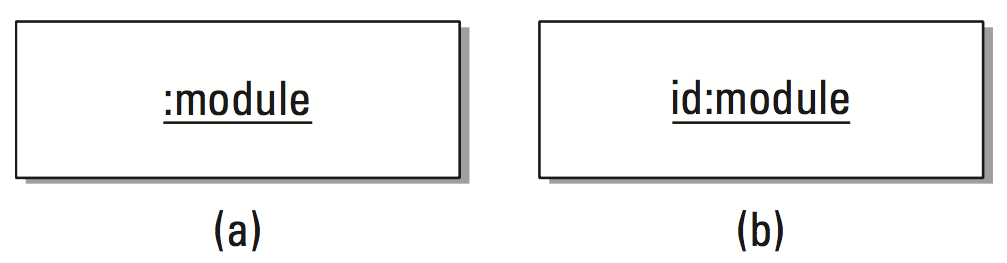
\includegraphics[width=0.7\textwidth]{img/f3-2.png}
	\caption{}
	\label{fig:f3-2}
\end{figure}

\begin{figure}[h] \centering
	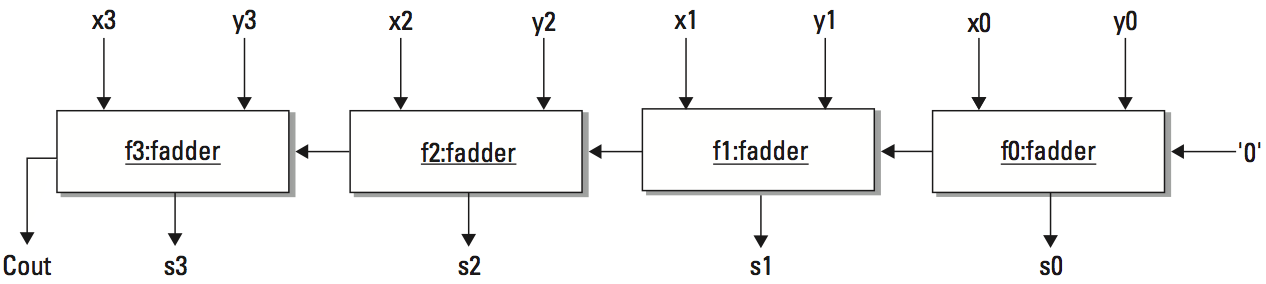
\includegraphics[width=0.9\textwidth]{img/f3-3.png}
	\caption{}
	\label{fig:f3-3}
\end{figure}

Tendo em mente todos estes conceitos, é possível descrever conceitos mais amplos no tema de \textit{design} de sistema.



\subsection{Abstração e Estado}

Abstração é definido no dicionário como operação intelectual em que um objeto de reflexão é isolado de fatores que comumente lhe estão relacionados na realidade, ou seja, tirar fora, extrair, remover. Assim, uma abstração é a arte ou um artifício de abstrair ou retirar. Dessa forma, um módulo é uma abstração de alguma funcionalidade em um sistema. Um módulo se torna uma boa abstração se suas interfaces e descrições provêm um fácil compreensão. Mas isso torna sua implementação mais complexa. Uma boa abstração capta todas características importantes e elimina tudo que não é importante para a ideia, ou seja cria uma organização. Uma imagem rica em informação pode não ser tão relevante imediatamente. Se isso for uma abstração ruim de algo, forçará-nos a pensar não sobre a singularidade do módulo, mas também como foi implementado, o que não é uma informação valiosa para uma abstração.

Estado já são uma palavra bastante conhecida no âmbito de sistemas eletrônicos. Eles são explicitados num \textit{design} de máquinas sequenciais e podem ser um ponto de memória de dispositivos eletrônicos como flip-flops. Já em sistemas embarcados, sua definição é um pouco mais abstrata já que um estado de módulo pode ser armazenado em vários lugares em várias formas distintas como flip-flops, static RAM, arquivo, ou até mesmo off-chip. Sendo assim, estado é uma condição de memória onde é possível segurar uma informação por um certo período de tempo.


\subsection{Coesão e Acoplamento}

Dessa forma, pra conceitos temos abstração e estado e pra mensuração teremos coesão e acoplamento. Coesão é uma métrica de abstração. Se os detalhes dentro de um módulo no ato da implementação são funcionalidades compreendidas facilmente, então o módulo possui coesão. O acoplamento é a forma de como os módulos estão relacionados uns com os outros. Uma dependência entre módulos é quando um comunica diretamente com outro. Quando um módulo A invoca um módulo B, então A depende de B. Mas B não necessariamente depende de A. Entretanto, dependência não é sempre explícita e com isso a o conceito estado entra em ação para auxiliar na formação de um módulo. Um exemplo disso é quando dois módulos parecem não ter nenhuma dependência entre si, mas que o sistema exige que ambos tenham terminado uma tarefa no mesmo tempo, criando assim uma dependência e consequentemente o sistema é acoplado no quesito tempo. Dependências não é algo ruim. São necessárias para que o procedimento possa funcionar corretamente com todos os outros módulos, mas precisa-se saber também o grau de acoplamento no sistema sendo essa em número e tipo. Dependência surgidas a partir de interfaces formais são as melhores formas de dependências. Uma forma de reduzir acoplamento em sistemas são por meio de encapsulamentos. Tais envolvem manipulações de estado e introdução à interface formal. A ideia é mover um estado dentro de um módulo e fazer com que isso seja exclusivo dele, também chamado de informação escondida. Isso permite uma maior liberdade de mudança interna no módulo já que a mudança de formatos de um estado não introduz um erro em outro e se o módulo possui uma boa abstração, então a informação escondida também permite que ele seja implementado de forma isolada. Assim, acoplamento é o resultado de dependências entre módulos.

É preciso evitar acoplamentos quando desnecessário e para isso existem várias técnicas para manipulação do grau de acoplamento.

É possível ver na Figura \ref{fig:f3-4} (a) que os submódulos B e C possuem dependência do módulo somatório A. Na Figura \ref{fig:f3-4} (b) a somatória A é duplicada dentro de cada submódulo eliminando cada uma das dependências existentes.

\begin{figure}[h] \centering
	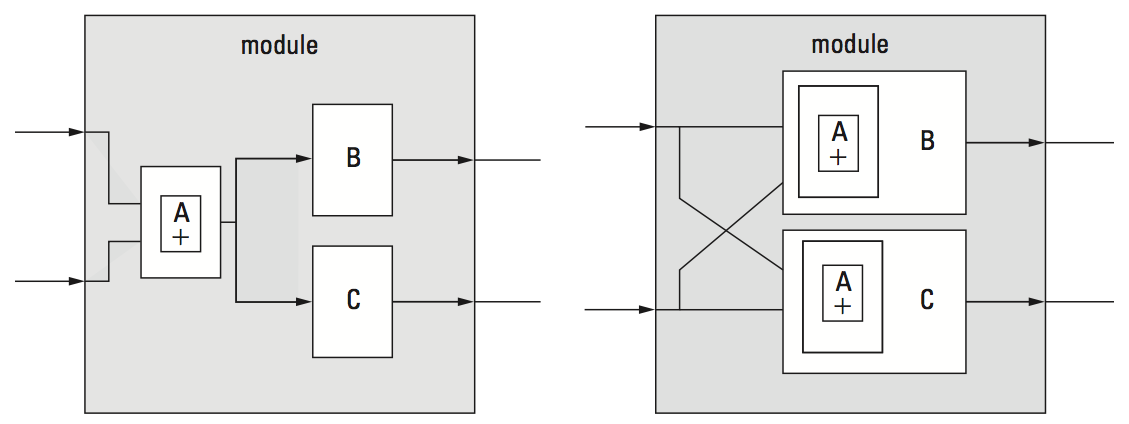
\includegraphics[width=0.8\textwidth]{img/f3-4.png}
	\caption{}
	\label{fig:f3-4}
\end{figure}

Será proposta uma situação exibindo o porquê desta abordagem pode ter mais vantagens: suponha que A foi \textit{design}ado para calcular somente números não-sinalizados. Mas com o passar do tempo, C necessita de operar com número sinalizados. Dessa forma, na Figura xa o \textit{design} deveria alterar tanto C quanto A. Alterando A, obrigatoriamente afetará B. Mesmo que B continue a trabalhar bem com a alteração de A, ouve uma cascata de alterações a serem feitas ao longo do tempo sobre algo que deveria ser pequeno, simples e isolado.

Discutindo sobre desvantagens deste procedimento, talvez se pensa que isso pode aumentar no tamanho do \textit{design} do projeto já que está duplicando um item, mas não. É possível que a funcionalidade de A seja simplesmente mesclado com o configurable logic block (CLB) já alocado para os submódulos B e C e consequentemente é possível que não haja nenhum ganho de conexão no CLB alocado. É claro que isso não é sempre verdade e é possível sim que tenha aumento de custo. Uma segunda desvantagem é, ao duplicar um módulo, agora se tem o mesmo componente em dois lugares. Se um erro for encontrado em um, deverá ser alterado noutro também.

\subsection{Planejando para o Reuso}

Além de qualidade, outro princípio é o torná-lo reusável. Com o constante aumento de complexidade dos componentes, é imprescindível que construamos \textit{design}s com intenção de serem reutilizáveis. Primeiramente é necessário criar e identificar \textit{design}s reutilizáveis. Alta coesão e baixo acoplamento são indicativos de componentes reutilizáveis. Existem custos em escondidos por meio de relative cost of reuse (RCR) e relative cost of writing for reuse (RCWR) e eles serão dissertados a seguir.

RCR são custos que fazem com que tenhamos que ler a documentação para entender como utilizar o módulo e o RCWR é o esforço extra que alguém deve exercer para projetar um módulo que outros possam utilizar (POULIN ET AL, 1993). Um exemplo é o \textit{trade-off} de aprender a utilizar a função strcpy da biblioteca string.h contra o tempo de criar a nossa própria função de cópia. Em alguns casos, poderia ser fácil gerar nosso próprio a invés de aprender um componente potencialmente complexo. Isso provavelmente seria por causa do alto RCR do módulo.

Uma forma de gerenciar o RCWR é tomar uma abordagem incremental onde é projetado um componente específico no \textit{design} atual. Se ele for necessário novamente, copie e generalize-o. Para vários \textit{design}s, adicionar uma generalização torna o componente reusável. Em linguagem VHDL, isso pode ser conseguindo introduzindo generics no projeto. Um ponto importante de máquinas computacionais personalizadas são a vantagem de serem específicas. Simplesmente adicionando generalização sem deixar a opção de gerar versões específicas de aplicativos através de genéricos é improdutivo. Refatoração é a tarefa de procurar em um \textit{design} existente e rearranjar os agrupamentos e hierarquia sem alterar sua funcionalidade, como é exibido muito bem na Figura \ref{fig:f3-4} e é feito para fazer componentes reutilizáveis. É possível que haja situações onde a refatoração pode acidentalmente alterar a sua funcionalidade. Para isso existe o processo de teste regressivo. Ele é usado para prevenir tal situação. Geralmente é automatizado e ser uma simulação dirigida tal como os testsbenchs já comumente conhecidos ou mesmo uma série de sistemas que contornam o componente exercitando sua própria funcionalidade. São necessários vários sistemas pelo fato de quererem também testar todos os genéricos que estão no conjunto em tempo de compilação.


\section{Gráfico de Controle de Fluxo}

É possível ver que os detalhes abordados aqui são referenciados a um \textit{design} de \textit{software}. É possível representar um sistema, quanto em \textit{software} ou em \textit{hardware}, de várias formas. Uma delas é o desenvolvimento de rápidos protótipos e este é referenciado como um \textit{design} de referencia de \textit{software}. Por mais que o custo de sua criação é algo ruim, sua forma de especificação sistêmica traz várias vantagens. A mais notável é a generalização de uma especificação bastante completa, sendo qualquer dúvida sobre o comportamento do sistema, é possível olhar no \textit{design} referencial. E sendo é um projeto que pode ser lido pelo computador, a sua especificação pode ser analisada por ferramentas computacionais.

Assumindo que o \textit{design} de referência de \textit{software} já exista, será mostrado como este pode ser demonstrado matematicamente e auxiliar-nos em o que deve ser implementado em nível de \textit{hardware} ou \textit{software}. Pra isso, utilizar-se-á o gráfico de controle de fluxo (CFG). Ele é definido por $ G = (V, E) $ onde V são vértices que representam os blocos básicos e as arestas indicam a todas as possibilidades de caminhos. Um bloco básico é uma sequência maximal de instruções sequenciais com \textit{single entry and single exit} (SESE).

\begin{figure}[h] \centering
	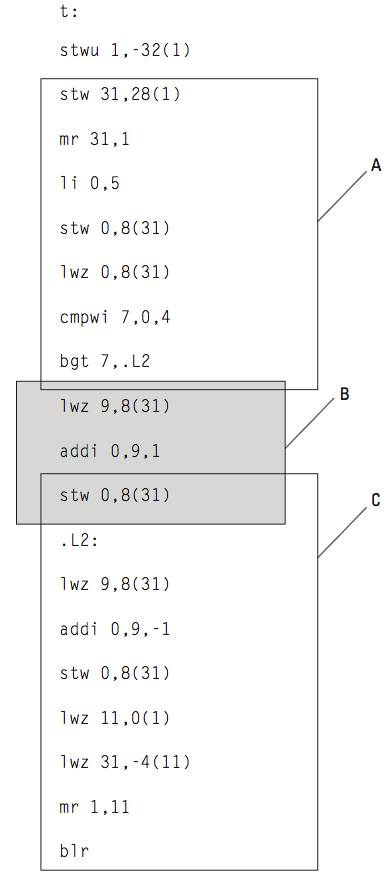
\includegraphics[width=0.5\textwidth]{img/f3-5.png}
	\caption{}
	\label{fig:f3-5}
\end{figure}

O primeiro grupo A é um bloco não básico porque não é maximal, ou seja, a primeira instrução store word with update deveria estar incluída. Grupo B é um bloco básico. Já o grupo C não é pois tem duas entradas para o bloco sendo elas no store word e também pelo branching para L2.

\begin{figure}[h] \centering
	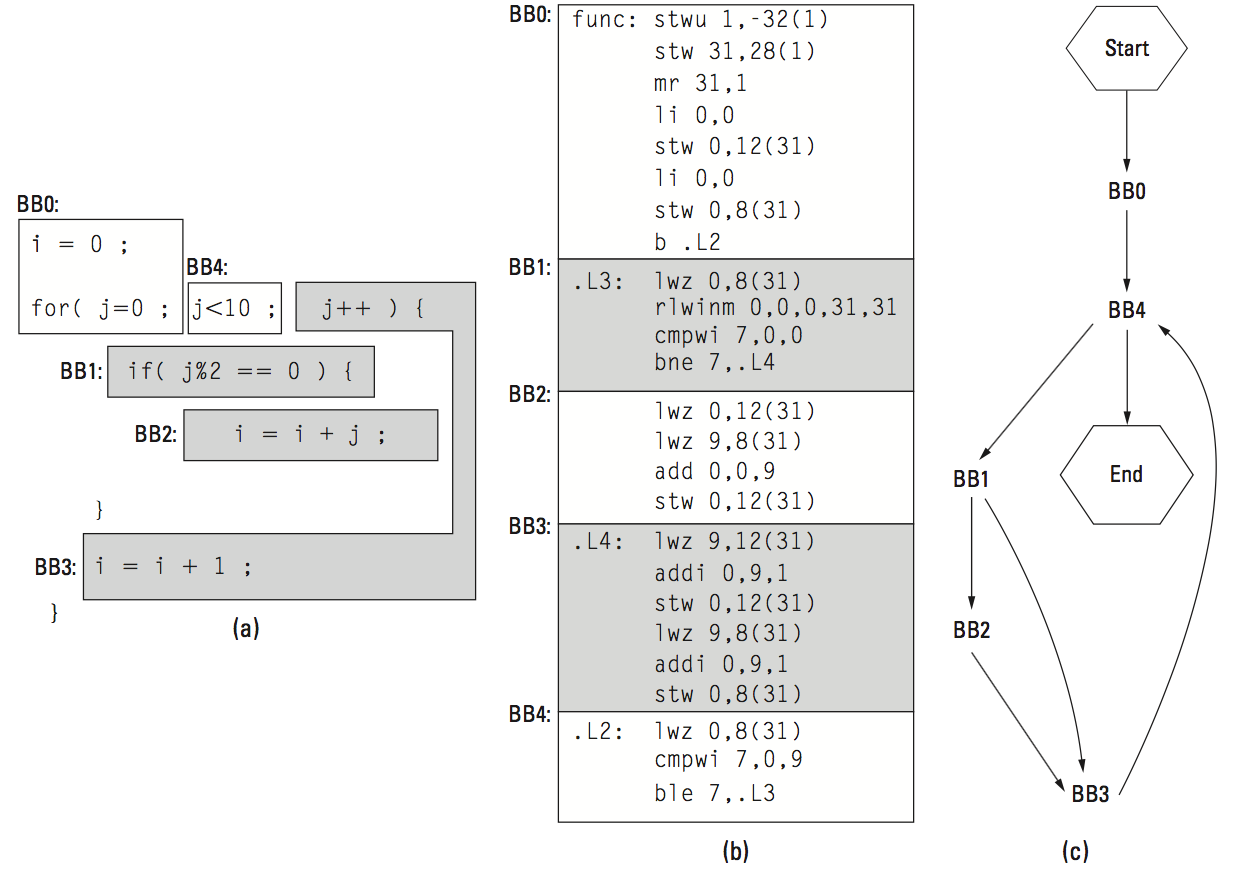
\includegraphics[width=0.8\textwidth]{img/f3-6.png}
	\caption{}
	\label{fig:f3-6}
\end{figure}

A Figura \ref{fig:f3-6} (a) exibe os blocos básicos em um código em alto nível. A Figura \ref{fig:f3-6} (b) exibe os o código gerado por um compilador para PowerPC onde os blocos básicos também são identificados e por fim o gráfico de controle de fluxo. Sabe-se que, é só possível identificar o bloco básico em C desde que se sabe como compilador foi  utilizado para gerar código, o que não acontece com assembly já que é possível identificar os blocos já com as próprias instruções.


\section{Design de \textit{Hardware}}

Até agora foi discutido os tópicos de modo genérico. A partir de agora, a discussão terá foco em \textit{design} em \textit{hardware}, em especial \textit{design} à Plataforma FPGA.

Designers raramente queriam construir em sistemas embarcados a partir de simples rabiscos e para isso utilizavam arquiteturas já existentes removendo componentes desnecessários e então adicionando cores aos requisitos do projetos. O modelo processador-memória, exibido na Figura \ref{fig:f3-8}, teve grande sucesso no início. Isso se tornou possível por causa da popularização do IBM Personal Computer em 80. Isso impulsionou desenvolvedores terceiros a criarem periféricos e máquinas compatíveis com outros fabricantes. E como a demanda aumentava com o passar do tempo, foi possível que os fabricantes pudessem tentar diferentes \textit{design}s de arquiteturas de computadores.

\begin{figure}[h] \centering
	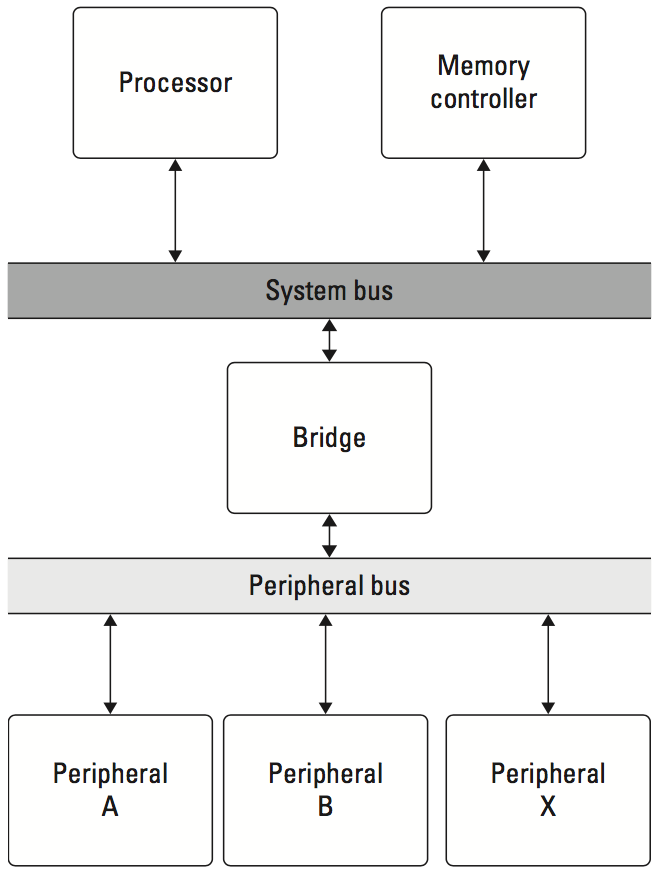
\includegraphics[width=0.5\textwidth]{img/f3-8.png}
	\caption{}
	\label{fig:f3-8}
\end{figure}

Computação embarcada não tinha grandes mudanças desde então, pois como é possível ver na Figura \ref{fig:f3-8}, esta arquitetura permitia o aprimoramento de componentes individuais do sistema. Por mais que o sistema de barramento seja insuficiente, ele serve bem para aplicações em geral e esse sistema é um bom ponto inicial para um \textit{design} em Plataforma FPGA. A Plataforma FPGA tem adota este tipo de arquitetura pois provê um framework estável que pode ser construído sobre \textit{design}s customizados. É possível construir complexos sistemas utilizando componentes existentes e cores, e com tempo reduzido em relação a sistemas embarcados tradicionais.


\subsection{Componentes de uma Plataforma FPGA}

Com a ideia de modularidade, coesão, casamento de componentes e \textit{design}, queremos iniciar uma construção de um sistema base que pode ser reutilizado como ponto de partida para um projeto de sistema embarcado, sendo este o modelo processador-memória.

O processador oferece controle e um ambiente de \textit{design} familiar ao \textit{\textit{design}er}. Mesmo que use pouca ou nenhuma relação com processadores, é usado para uma rápida prototipação. Pode existir dois tipos de processadores, os processadores \textit{hardware} e \textit{software} core, sendo o processador hard já é bem conhecido. Algumas Plataformas FPGA provê recursos reconfiguráveis suficientes para que um processador \textit{soft} possa ser implementado em blocos lógicos. Eles fornecem flexibilidade e são naturalmente configuráveis. Inicialmente, mesmo processadores básicos, precisam de alguns recursos básicos e tal forma se chama stand-alone.

Antes da implementação de fato, é preciso verificar se o FPGA já possui um processador \textit{hardware}, se possui recursos suficientes para a implementação de um, qual o papel do processador e o \textit{software} será utilizado nele e isso será discutido ao decorrer deste.

A memória pode ser organizada e hierarquizada de várias formas diferentes como Von Neumann ou Harvard, ou mesmo com níveis de caches diferentes. Tal como o processador, deve-se perguntar que tipos de memórias estão disponíveis, quanto há disponível e outros parâmetros de implementação. Em um sistema, ela pode ser considerada como um componente, um core, ou uma parte básica e sua localização determina a interface e acessibilidade. Um controlador de memória é requerido para controlar as transações de memórias. O uso eficiente é o item mais crítico pois ela pode gerar lags com o processador.

\subsubsection{Barramento}

As interfaces de cada componente, como o processador e memória, se conectam via barramento padronizado. Um core que pode requisitar acesso é considerado barramento master, o que demonstra que nem todos os cores necessitam de ser master, o que tornam barramento \textit{slave}. Um barramento no FPGA é implementado em lógica configurável, o que torna um \textit{soft} core. Detalhes importantes são quais cores necessitam de comunicar diretamente, alguns comunicam mais frequentemente ou necessitam de uma alta vazão.

Geralmente, o barramento com maior vazão é o que fornece a conexão entre processador e controlador de memória e geralmente é o primeiro barramento a ser adicionado ao projeto. Um segundo pode ser adicionado para separar o \textit{design} em diferentes domínios, geralmente em \textit{low} e \textit{high-speed} ou com largura de banda dedicada à comunicação. Esses são conhecidos como barramento de periféricos. Utilizando barramentos simples, para realizar uma operação na memória, deve-se realizar uma requisição e o múltiplos barramentos permitem a comunicação paralela.

Quando necessita de uma comunicação de um core com um periférico, utiliza-se de um bridge. É um core especial que resite em ambos os barramentos e propaga requisições de um barramento para outro. Trata-se de uma interface que funciona como um barramento mestre em um barramento e um barramento \textit{\textit{slave}} em outro e assim o \textit{\textit{slave}} responde à requisição que deve ser passada a outros os periféricos. Geralmente somente uma bridge simples é requerida, onde todos os periféricos são conectados nela, tendo um sistema de bridge para gerenciamento das solicitações e respostas.


\subsubsection{Periféricos}

Quando se menciona periféricos, geralmente é referido à \textit{hardware}s cores como impressoras, LCDs, GPSs e outros. Periféricos pode-se de dizer que são todos os componentes que estão em torno à unidade de processamento central. Todos eles possuem algum tipo de interface de comunicação, sendo ela uma PCI Bridge, Ethernet, USB, UART, I$^2$C, SPI e muitos outros.


\subsubsection{O Sistema Base}

Pra início, será montado um sistema conceitual simples constituído de um processador, dois tipos de memória e uma comunicação UART. Como resultado, este conceito será base para vários outros tipos de \textit{design}s.


\begin{figure}[h] \centering
	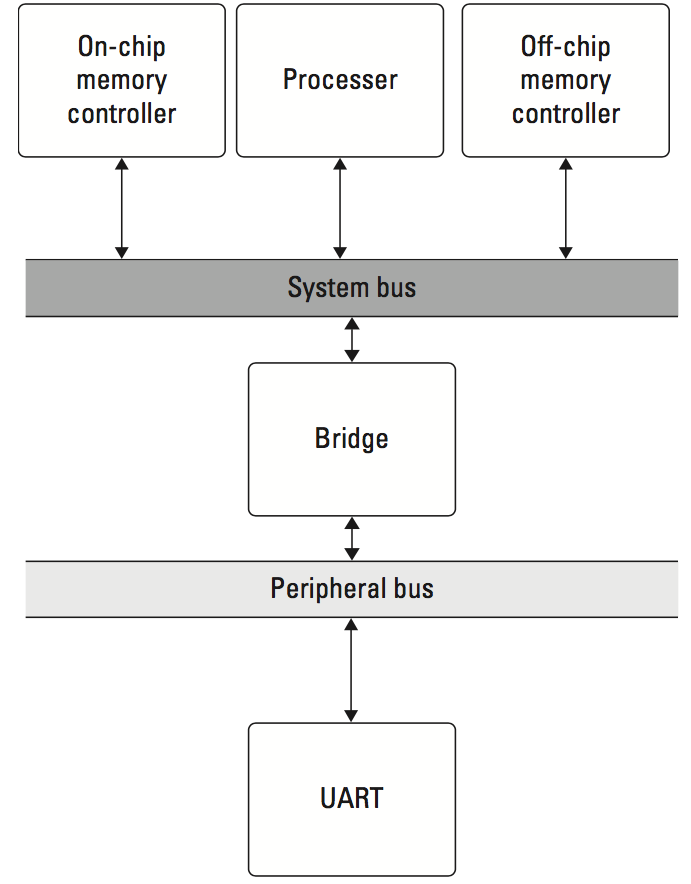
\includegraphics[width=0.5\textwidth]{img/f3-9.png}
	\caption{}
	\label{fig:f3-9}
\end{figure}

O benefício de utilizar dois sistemas de barramento é a facilidade de modificação ao adicionar e substituir componentes podendo assim termos o seguinte \textit{design} de sistema exibido na Figura \ref{fig:f3-10}, de acordo com nosso propósito.

\begin{figure}[h] \centering
	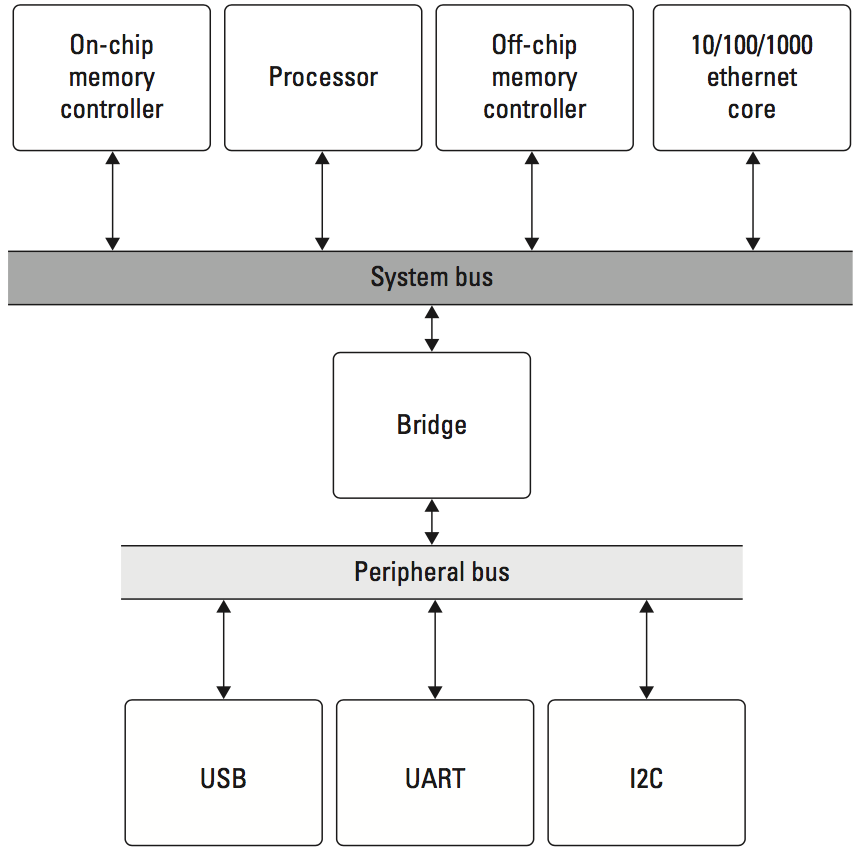
\includegraphics[width=0.7\textwidth]{img/f3-10.png}
	\caption{}
	\label{fig:f3-10}
\end{figure}

Em uma perspectiva de \textit{hardware}, a localização de dados é facilmente identificável. Memória off-chip é um modo separado e seu acesso é nada mais que seus endereços. O endereçamento é importante para qualquer core possa comunicar com o processador. A Figura \ref{fig:f3-11} mostra o mapa de endereçamento dos dois barramentos. Cara core possui um intervalo na memória é considerado um \textit{\textit{slave}} e o processador não possui um espaço de memória no mapa. Em sistemas com dois barramentos, o bridge atua como um intermediário entre as requisições e o sistema de barramento periférico.

\begin{figure}[h] \centering
	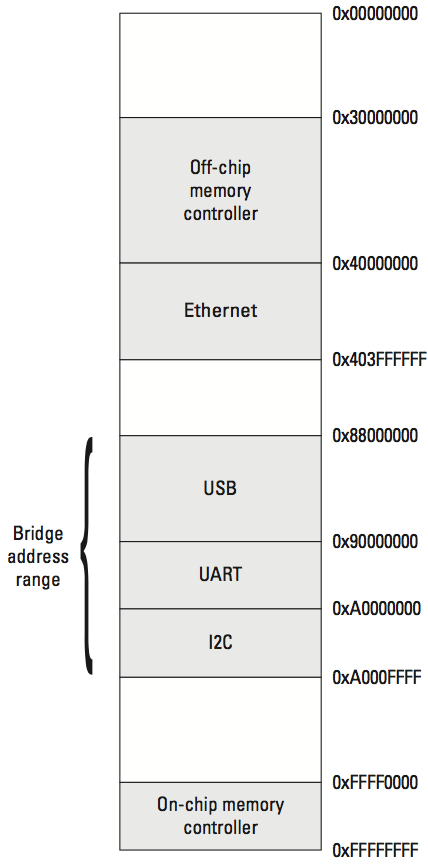
\includegraphics[width=0.5\textwidth]{img/f3-11.png}
	\caption{}
	\label{fig:f3-11}
\end{figure}

\subsection{Montando Sistemas Personalizados}

Para iniciar, deve-se responder a pergunta de porque construir um sistema personalizado. Acreditava-se que desenvolvimento de \textit{hardware} é um processo difícil porque existem mão de obra para \textit{software}s profissionais do que engenheiros de \textit{hardware}. E a resposta para a pergunta ‘porque desenvolver um \textit{hardware}’ é para obter performance além de eficiência e previsibilidade.

Sabendo-se que um FPGA não terá o mesmo ganho que um processador projetado já em silício, deve-se analisar como o \textit{hardware} FPGA supera um processador. Existem duas razões porque alguns \textit{design}s de FPGA possuem vantagens em performance. A primeira é sobre o modelo de execução. O modelo de computação sequencial von Neumann possui uma barreira em sua performance por causa do fato de expressar suas tarefas como um conjunto sequencial de operandos. Em \textit{hardware}, o paralelismo inerente da tarefa pode ser expressado diretamente. Para compensar sua operação serial inerente, processadores modernos possuem uma porção significante de recursos de \textit{hardware} para extrair em nível de instruções o paralelismo como estratégia de aumentar a vazão. Para algumas aplicações, largura de banda de memória limita a performance e parte da banda é consumida pelas instruções sendo buscadas, da memória e assim, instruções fazem parte implícita do \textit{design}. A segunda razão é que FPGA pode ter uma especialização. Em processadores de propósito \textit{data path} e tamanho de operações são organizados por meio de requerimentos gerais. Isso significa que, para multiplicar um inteiro por uma constante $ c $ é necessário de um multiplicador completo no sistema. Se essa informação já é conhecida, uma implementação baseada em FPGA pode ser criada com funções personalizadas.

Supondo que uma implementação em \textit{hardware} de uma tarefa A leva o mesmo tempo a ser executada no processador e ambas são de fácil implementação e questiona-se se ainda é viável a implementação desta. A resposta é sim quando a solução em \textit{hardware} é mais eficiente. Eficiência é definida como facilidade de realizar uma tarefa fixa com uma quantidade variável de recurso sendo recurso a área de prototipação, número discreto de chips, ou o custo da solução. Um \textit{hardware} personalizado e um processador possuem são mais eficientes que dois processadores.

É possível também o caso de um processador não ser totalmente utilizado de sua capacidade. Mesmo utilizando a propriedade de multitarefa em novas funcionalidades, existem razões para escolher a implementação. Alguns casos faz sentido mover uma tarefa para o \textit{hardware} se a torna mais previsível ou se torna o escalonamento no processador mais facilitado. Em casos onde restrição de tempo é importante, como sistemas de tempo real, a meta é satisfazer as restrições e assim previsibilidade é mais importante que performance. Entretanto, a única desvantagem de desenvolver em \textit{hardware}, como já mencionado é o esforço requerido. O número de engenheiros de \textit{hardware} é relativamente baixo comparado com profissionais que desenvolvem em \textit{software}. Desenvolvimento em \textit{hardware} não mais difícil que em \textit{software}, mas sim, necessita de atenção no projeto. Em resumo, uma Plataforma FPGA oferece vantagens de performance, eficiência e previsibilidade sobre soluções somente em \textit{software}. Como um projetista de FPGA, parte de sua tarefa inclui determinar quando um simples controlador é apropriado.


\subsubsection{Composição de \textit{design}}

Existem três passos para fazer um \textit{design} de um core modular customizado. O primeiro passo é identificar as entradas e saídas, onde em muitos casos estas são baseadas em suas funcionalidades. O segundo é identificar os operandos e compor o \textit{data path}, geralmente uma coleção de computações de multiestágios (isto é, \textit{pipeline}). Cada componente é \textit{design}ado a uma funcionalidade particular. Os operando exatos podem não ser claros no início da fase de \textit{design}, mas determinando a funcionalidade em baixo nível necessárias permite a construção de um \textit{data path}. Um \textit{data path} representa o fluxo de dados por meio do componente. Uma vez definido, é possível construir o \textit{pipeline}, no qual contribui com a performance e eficiência do \textit{design}. Capturando os estágios do \textit{pipeline} pode ser árduo inicialmente, mas iniciando um \textit{design} com o conceito de suporta à operações \textit{pipeline} faz com que o projeto seja mais gerenciável. O terceiro paço é o desenvolver o circuito de controle que sequencia as operações, frequentemente a máquina de estados finitos. Frequentemente referenciamos um \textit{hardware} em termos de paralelismo, onde cada operação é independente e podem ser executadas ao mesmo tempo. Com a máquina de estados finitos é possível gerenciar a computação executando as operações paralelas e em seguida as sequencias e dependentes.

Existem duas abordagens de \textit{design}, \textit{bottom-up} e \textit{top-down}. Em muitos casos, utiliza-se a abordagem \textit{bottom-up} no desenvolvimento em FPGA. Em método estrutural HDL, cada componente é construído por seus subcomponentes e assim, antes do \textit{top-level}, todos os subcomponentes devem ser construídos e testados. Nessa abordagem, cada subcomponente pode ser tratado como uma \textit{black-box} onde as entradas e saídas são conhecidas. Na abordagem \textit{top-down}, quando se quer desenvolver um core personalizado, o \textit{\textit{design}er} deve começar com as interfaces de entrada e saída, criando assim o início da \textit{black-box}. Uma vez definida, é possível decompor sistematicamente em subcomponentes. Esse processo repete até os blocos de baixo nível onde podem ser simples o suficiente. Esta abordagem não é associada a nenhum HDL estrutural ou comportamental, mas é possível utilizada com o último.

Em ambas as abordagens, internamente podem ser construídas de formas distintas, mas no final todas possuem a mesma funcionalidade. Considere o seguinte componente somador de quatro números da Figura \ref{fig:f3-12}. Na implementação temporal da Figura \ref{fig:f3-13} existe um multiplexador que realizará a soma de acordo com o controlador da máquina de estados finitos. A máquina de estados finitos terá quatro estados ao todo e percorrerá de forma sequencial. Utilizando somente uma ALU e um registrador, temos o circuito que utiliza menor quantidade de recursos possível, mas não temos a solução com menor tempo. Para aumentar o speed-up, devemos considerar a abordagem paralela e adicionar mais recursos. Um sistema com três ALUs poderá realizar as operações \texttt{temp1 = a + b}, \texttt{temp2 = c + d} e \texttt{temp1 + temp2}. O \textit{trade-off}, da latência e recursos fica a cargo do \textit{\textit{design}er}.

\begin{figure}[h] \centering
	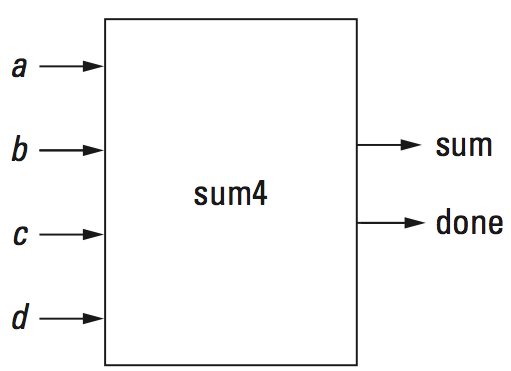
\includegraphics[width=0.5\textwidth]{img/f3-12.png}
	\caption{}
	\label{fig:f3-12}
\end{figure}

\begin{figure}[h] \centering
	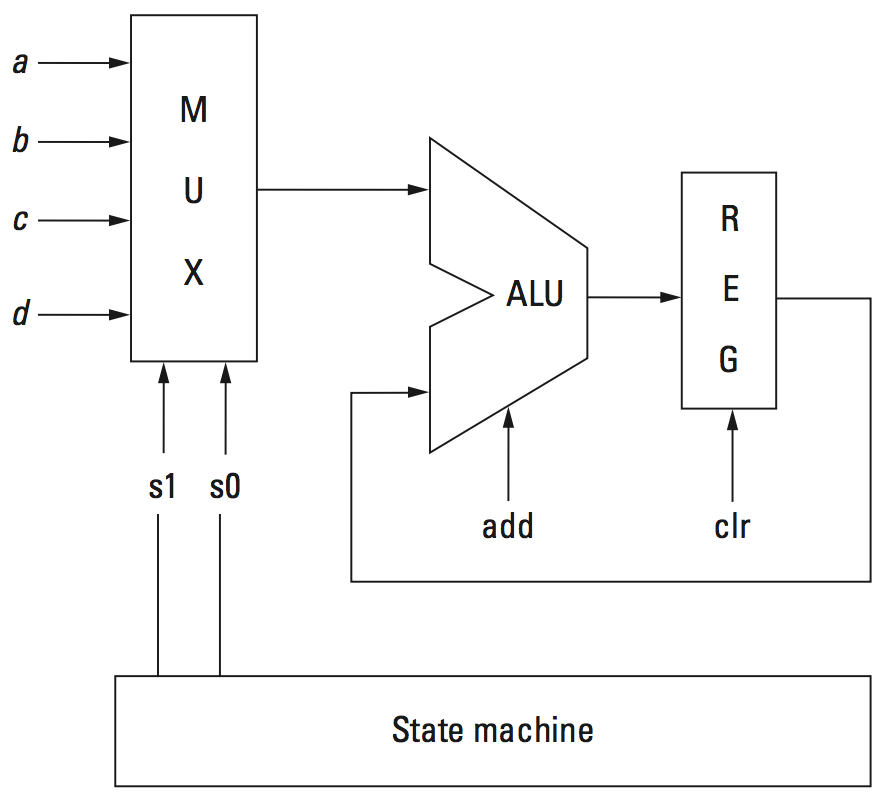
\includegraphics[width=0.5\textwidth]{img/f3-13.png}
	\caption{}
	\label{fig:f3-13}
\end{figure}

Quando existem operações sequencias, implica que existe um controle onde a segunda toma lugar em seguida da primeira após sua computação e isso degrada no caso de composição espacial o que diminui a estrita ordenação de operações. Dessa forma, quando um \textit{hardware} especifica duas operações, elas serão executadas simultaneamente ao menos que o \textit{\textit{design}er} tenha especificado previamente uma ordem. A Figura \ref{fig:f3-14} mostra a implementação espacial do somador. Nesse caso, as operações de adição são \textit{pipeline} tais que os resultados são alimentados para frente para o próximo somador. E execução solta em FPGA pode gerar vantagens e desvantagens. A concorrência é o que fornece ao sistema performance, e controle do tempo é o que fornece previsibilidade. Expressar simplesmente relações de tempo entre operações é um desafio.

\begin{figure}[h] \centering
	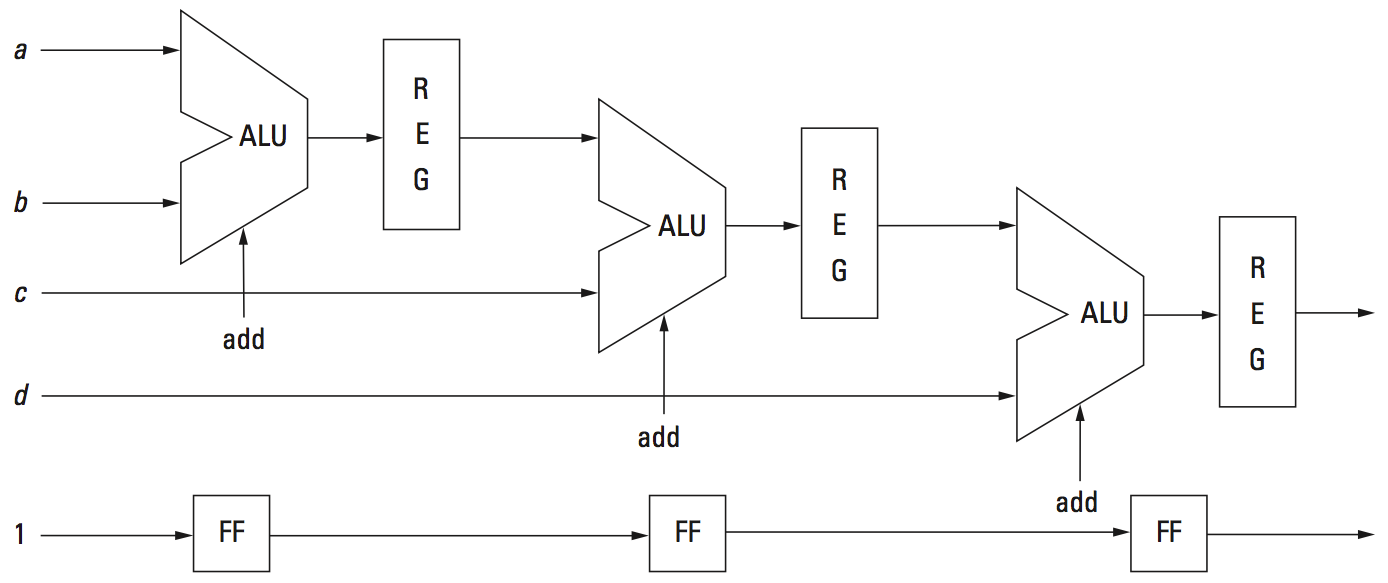
\includegraphics[width=0.8\textwidth]{img/f3-14.png}
	\caption{}
	\label{fig:f3-14}
\end{figure}


\section{Design de Software}

No passado, \textit{software} era simples. Tinham uma simples tarefa, e executava um papel relativamente menor comparado com o \textit{design} de \textit{software} da época. Se duas tarefas eram solicitadas, eram frequentemente deixadas independentes, lógico e fisicamente. Com microcontroladores tornando mais veloz, sistemas embarcados adicionaram sistemas de \textit{software} para gerenciar controle de múltiplas tarefas. Isso permite quem um microcontrolador simples possa fazer a multiplexação de tarefas separadas por tempo. Em sistemas embutidos atuais, seus processadores possuem unidade de gerenciamento de memória, suporte de memória virtual e com tecnologia suficiente para suportar sistemas operacionais. Tais características são tidas como vantagens pois resulta em uma explosão de novas características e assim permitindo a incorporação e adaptação de aplicações de \textit{software}s grandes que originalmente eram escritos para computadores de propósito geral e máquinas servidoras.


\subsection{Opções de Sistema de Software}

Um desenvolvimento de um sistema embarcado possui vasto escolhas quando vem para sistema de \textit{software}. Sistema de Software referimos a qualquer \textit{software} que assista a aplicação, geralmente adicionando uma interface em \textit{software} para acesso ao \textit{hardware}. Isso segue desde simples bibliotecas de rotinas até sistemas operacionais totalmente desenvolvidos que virtualizam o \textit{hardware} para processos individuais. Em muitos os casos, não é necessário um sistema de \textit{software}. Nesses casos, os arquivos iniciais executados antes do \texttt{main} em C, por exemplo, são modificados. Sem um sistema operacional, essas rotinas são responsáveis por definir o estado inicial do processador e periféricos. Mesmo que o processador tenha uma unidade de controle de memória,  simples casos que a aplicação executa em modo real e privilegiado, nenhuma proteção de memória é utilizado. Isso se chama programa standalone C, pois executa sem nenhum sistema de \textit{software} adicional e com isso, tem uma abordagem de sistema simples.

Para FPGA, isso é frequentemente o primeiro passo quando se testa um novo \textit{hardware} core, pois um programa em C tem total acesso ao \textit{hardware}. Geralmente, essa solução produz um executável suficientemente pequeno que o sistema de \textit{software} inteiro pode ajustar dentro de um bloco de memória RAM no FPGA. A desvantagem é a necessidade de desenvolvimento. Não á proteção contra erros de \textit{software}. Talvez o grande retrocesso hoje é que é difícil ter vantagem de \textit{software} existente que assume que admite uma biblioteca C completa e um \textit{workstation}. As vezes a adição de funcionalidades de um sistema de \textit{software} como o suporte a multithreads pode ser útil, diferente da indesejável sobrecarga ao adicionar recursos completos de um sistema operacional. Vários produtos e soluções Open-Source são feitos para sistemas embutidos.

Um passo acima de standalone é uma simples biblioteca de threads. Sistemas operacionais provem um número de serviços para uma aplicação, mas isso tem um custo. Os sistemas operacionais de sistemas embarcados são diferentes dos utilizados nos desktops, significando que o desenvolvedor tem que aprender novas interfaces, convenções e o que está ou não disponível. Analisando de forma espectral, em um lado tem-se um sistema operacional com recursos completos, utilizados por \textit{\textit{workstation}s}. A maioria dos sistemas de \textit{software} descritos podem ser executados sem um subsistema de armazenamento secundário, ou seja, um sistema de arquivo. Entretanto, sistemas completos necessitam, no mínimo, sistema de arquivo raiz. Até recentemente, era inviável pensar em um sistema operacional completo em um sistema embarcado por causa de recursos requeridos. Entretanto, com novos dispositivos como a Plataforma FPGA isso se torna mais comum. Quanto mais serviços é colocado mais peso é adicionado ao desenvolvedor em saber o que é provido num sistema de \textit{software} e saber usá-lo. Com sistemas completos, os programadores já estão familiarizados com estes. Como sistemas operacionais são comuns, existem várias aplicações disponíveis. Com os sistemas embarcados se tornando mais obliquo e conectado à internet, eles necessitam suportar mais interfaces e mais protocolos de comunicação, o que o sistema operacional completo já fornece.


\subsection{Monitores e Bootloaders}

Nos primeiros microprocessadores baseado em sistemas embarcados, simples 8-bit migraram de computadores de hobbies e games para outros produtos comercias que agora chamamos de sistemas embarcados. Fabricantes desses microprocessadores geralmente desenvolvem kits que incluem board fabricadas que aumentam as capacidades dos chips e uma Board Support Package (BSP) que inclui compiladores, \textit{software} power-on-self-test (POST), bibliotecas de \textit{software} de Basic Input/Output System (BIOS) e um debugger. POST é executado antes de qualquer outro \textit{software} para verificações de que nada foi esgotado desde a última vez que foi ligado. Usando sub-rotinas da BIOS, o tamanho da aplicação continua pequeno.

Monitor é um simples \textit{software} de tipo primitivo ao debug. Debuggers modernos executam em um processo separado, tem acesso à tabela de símbolos do compilador e fornece uma rica e flexível interface. Ao contrário, um monitor é um driver de interrupção e suporta algumas funcionalidades básicas. Monitores tinham uma funcionalidade que não existem nos debuggers atuais, no qual suporta a transferência de memória sobre canal de comunicação serial transmitindo ASCII usado para interação. Como os caracteres ASCII possuem 7 bits e executáveis utilizam tudo como 8-bits de um byte, blocos de memória foram codificados para a transmissão. Enquanto é desenvolvido a aplicação, o \textit{\textit{design}er} poderia iniciar o monitor e copiar a aplicação para a RAM, ajudando o curto teste/debug dos \textit{software}s. Isso é importante pois, até o GNU debugger (ou gdb) possui subsistemas capazes de comportar como monitores.

Sistemas modernos moveram um passo a diante. Uma moderna substituição de um monitor pode ser a interface joint test action group (JTAG). Tal controlador gerencia qualquer endereço físico, incluindo a memória principal, provendo uma alternativa a abordagem dita dos monitores. Nesse caso, o debugger comunica com uma interface até o controlador JTAG. Da mesma forma as funcionalidades de POST/BIOS tem transformado em \textit{software} BIOS de desktops no qual inicia logo em seguida da energização do computador. Para alguns computadores, é critico que o BIOS coloque o computador e seus periféricos em um estado conhecido. Linux por exemplo não assume nada e permite que cada \textit{hardware} inicialize sozinho. Parcialmente concorrente com o desenvolvimento de PC, \textit{\textit{workstation}s} surgem com uma abordagem levemente diferente. Elas utilizam um pequeno \textit{software} chamado bootloader ou também chamado de PROM. Era simplesmente um programa que lia o primeiro setor de um disco, no qual contia outros programas mais avançados, e carregava-os para a memória principal, apontando o PC para o primeiro endereço desse setor. Esse então processava o carregamento do sistema operacional por completo. Essa técnica vem surgindo em PCs com boa aceitação. BIOS continua sendo o primeiro a ser executado, então o bootstrap é iniciado carregando o sistema operacional. Alguns conhecidos hoje são GRUB, U-Boot e o RedBoot.

Para sistemas embarcados, a abordagem BIOS/monitor ainda domina os pequenos microcontroladores e o legado sistêmico enquanto o bootloader está ganhando espaço em sistemas operacionais completos.

	\chapter{Particionamento}



\section{Visão Geral Sobre o Problema de Particionamento}

A decomposição de um design de referencial de \textit{\textit{software}} pode gerar dois componentes: uma porção a ser realizada em \textit{hardware} e outra executada em \textit{software}, num processador e isso é chamado de problema de particionamento. Para sistemas baseados em Plataformas FPGA, particionamento é um subproblema de um problema mais geral localizado no codesign de \textit{hardware} e \textit{software}. 

Para início, será considerado uma aplicação como um conjunto de instruções organizadas como uma coleção de grafos de fluxo de controle especificando a ordem de execução. Sendo assim, a ideia do particionamento é o grupo de específicos conjuntos de instruções em uma aplicação e então mapear esses grupos tanto em \textit{hardware} e \textit{software}. Os grupos designados ao \textit{software} são executados sequencialmente enquanto os mapeados em \textit{hardware} são implementados por uma combinação customizada ou por circuitos sequenciais. Se uma aplicação é totalmente funcional em design referencial de \textit{software}, o resultado do particionamento é conhecido como decomposição. Alguns fatores podem ajudar nas decisões de particionamento tal como expectativa de ganho de performance, os recursos utilizados em \textit{hardware}, como são usados e talvez o mais importante quanto de sobrecarga de comunicação a decomposição impõe ou dificuldade de implementar um conjunto específico em \textit{hardware}.

Recurso por definição são instruções de um \textit{cluster} conectado de aplicações de design referencial de \textit{software} adequado para uma implementação de \textit{hardware}. Adequado será utilizado para definir `o projetista do sistema antecipa que uma implementação de \textit{hardware} se mostrará vantajosa’. Para obter uma boa partição, geralmente tem que examinar grupos que podem ser maiores ou menores que sub-rotinas definidas pelo programador. Recurso pode variar de um pequeno conjunto de instruções para um \textit{kernel} de loops aninhados até um modulo de \textit{software} completo consistente de múltiplas sub-rotinas. Como o tamanho dos recursos afetam na performance, a decisão de implementação em \textit{hardware} depende da sua melhoria no sistema por inteiro e os recursos utilizados relativos a outros recursos candidatos. Se determinado a ser valido a pena, então os recursos de implementação em \textit{hardware} aumentam a arquitetura de \textit{hardware}. 

\textit{Profile}, também conhecido como recorte, é uma técnica para coletar informações em tempo de execução de uma aplicação. O \textit{software} referencial é executado com uma entrada representativa e o tempo gasto em várias partes da aplicação é mensurado. Um exemplo é exibido na Figura \ref{fig:f4-1} onde exibe a codificação de uma imagem.

\begin{figure}[h] \centering
	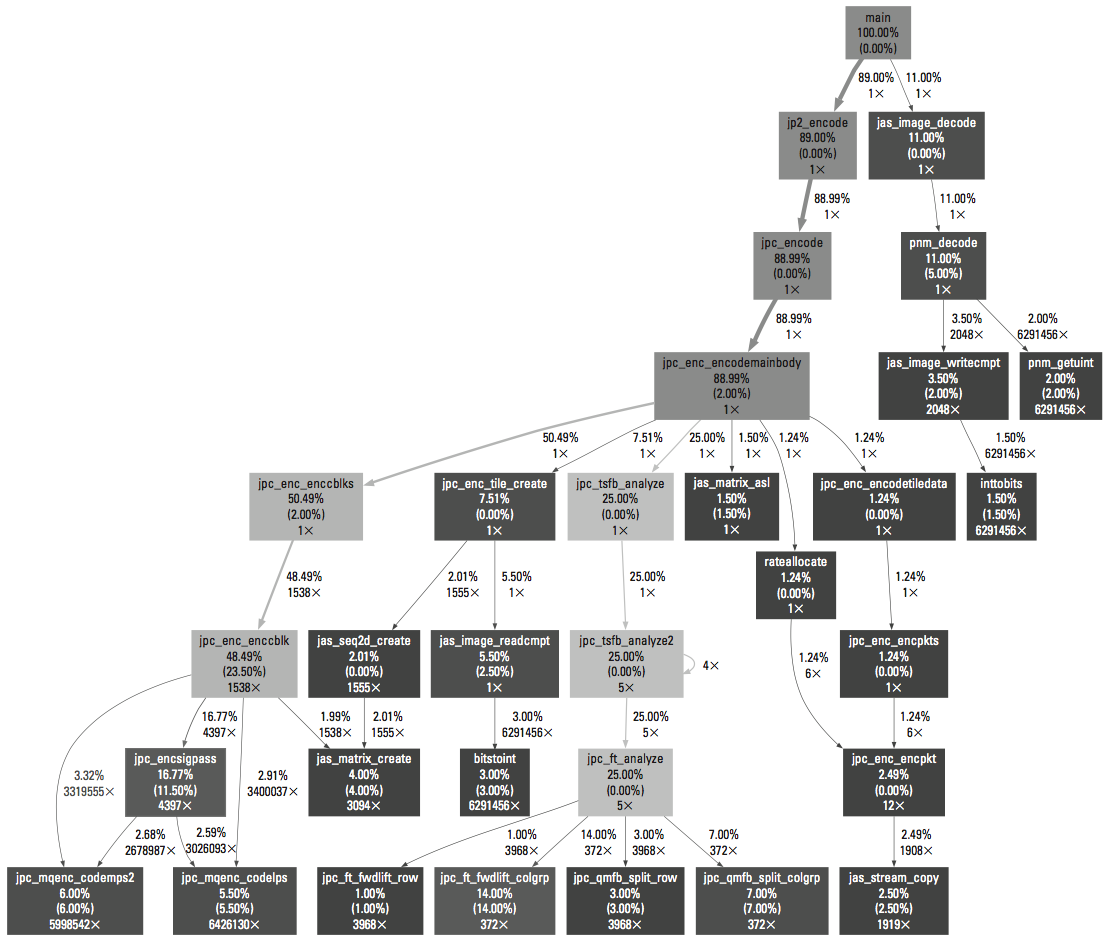
\includegraphics[width=0.9\textwidth]{img/f4-1.png}
	\caption{}
	\label{fig:f4-1}
\end{figure}

Aqui será assumido a técnica simplista que recortará uma aplicação por interrupção periódica e amostrar o \textit{program counter}. Um histograma pode ser utilizado para contar quando um programa é interrompido em um endereço particular e a partir desse, uma fração aproximada do tempo total de execução gasto em várias partes da aplicação pode ser computado.

A análise de performance é definida pela Lei de Amdahl que aplica a lei de retornos decrescentes à utilidade de uma única arquitetura, ou seja, 



$$ \text{Speed up}_{overall} = \frac{1}{(1 - \text{Fraction}_{enhanced}) + \frac{\text{Fraction}_{enhanced}}{\text{Speed up}_{enhanced}}} $$



articulando os limites de um melhoramento geral para uma aplicação que um simples realce pode fazer em tempo de execução. Generalizando para incluir todos os potenciais realces e métricas de performance arbitrária, pode-se caracterizar os limites como coleções de realce. Se forem em recursos de \textit{hardware} e pode-se antecipar que requer ganho potencial de recursos para cara tal, então pode-se desenvolver um modelo que irá orientar ao processo de particionamento. Tal lei não é adequada pois:
\begin{itemize}
\item Visa um simples realce e não nos auxilia a selecionar um subconjunto de uma coleção de recursos potenciais;
\item Foca somente no tempo de execução;
\item Não visa recursos requeridos;
\item Não visa custo de comunicações.
\end{itemize}

Perfis baseados em exemplos requerem representações de entrada e é uma aproximação de tempo gasto. Sem implementar todo o potencial de recursos em \textit{hardware}, pode ser difícil antecipar os recursos requeridos. Pode-se com determinação analítica calcular quantos ciclos de \textit{clock} um recurso de \textit{hardware} irá tomar, podendo assim calcular métricas como \textit{speed up}. Entretanto, é impossível saber quando um processo arbitrário será completado. Ao invés de prover uma solução automatizada, a solução analítica simplesmente provê um \textit{framework} para guiar um designer de sistema a criar uma solução criativa.



\section{Solução analítica para particionamento}

Para definir o problema, será descrito fórmulas matemáticas do problema de agrupamento de instruções em recursos e então os seus mapeamentos em \textit{hardware} ou \textit{software} e ao final, converter os recursos em implementações em FPGA. Atualmente, a forma mais comum de transcrever é descrever manualmente o core com um HDL utilizando design referencial de \textit{software} como especificação.

Muitos problemas práticos impactam na performance atual do sistema. Nem todos os problemas podem ser incorporados a um modelo analítico e por isso podemos caminhar no sentido de soluções matemáticas que irão produzir uma resposta aproximada ao problema de particionamento. Muitas das entradas do nosso modelo são estimadas ou aproximações no qual futuramente degrada a fidelidade de resultados. Deve-se importar com isso pois resolvendo o problema de particionamento `no papel’, tem-se um particionamento que é próximo ao ótimo. Daqui, cabe ao designer ser habilidoso em usar os guias e projetar uma solução mais refinada. Ao final, é mais eficiente usar uma combinação de técnicas \textit{ad hoc} e matemáticas para encontrar uma solução ótima do que simplesmente confiar numa intuição de engenheiro.

Para continuar, deve-se definir alguns conceitos básicos. Sabe-se já de antemão o modelamento de uma sub-rotina de um design referencial de \textit{software} utilizando o grafo de controle de fluxo (CFG) e além desse, será descrito uma nova notação para incluir o grafo de chamada (CG), no qual consiste num conjunto de CFGs, um por sub-rotinas 

$$ \mathcal{C} = {C_0, C_1, \dots C_{n-1}} $$ 

onde $ C_i = (B_i, F_i) $ é o CFG de uma sub-rotina $ i $. Sendo assim, a CG da aplicação é escrita por 

$$ \mathcal{A} \subseteq (\mathcal{C}, \mathcal{L}) $$ 

onde $ \mathcal{L} \in \mathcal{C} \times \mathcal{C} $. Duas sub-rotinas são relacionadas $ (C_i, C_j) pertence \mathcal{L} $ se podem ser determinadas no tempo de compilação que a sub-rotina $ i $ tem potencial de invocar a sub-rotina $ j $.

É assumido que os blocos básicos de cada sub-rotina são disjuntos, ou seja, cada bloco básico em uma aplicação pertence a exatamente um CFG. Além do mais, é assumido que um nó raiz para o CG é implícito, ou seja, uma sub-rotina é designada a iniciar a execução. Nem todos os executáveis podem ser expressados nesse modelo. O manuseio de sinais e interrupções não são representadas e assim, não é possível determinar todos vértices, $ F_i $ em uma dada sub-rotina $ C_i $ de um CFG antes da execução. Finalmente, o paradigma de orientação à objeto depende do tempo de execução para conectar os métodos virtuais invocados. Por design, esse paradigma nos previne de saber todos os vértices antes da execução. Para agora, será considerado que o modelo é suficiente para ser expressado em design referencial de \textit{software}. 

Um equívoco comum é que uma definição formal de particionamento só aplica a separação de aplicação componentes de \textit{hardware} e \textit{software}. Além do mais, para fazer o problema mais tratável é comum agrupar operandos de primeiro recurso, ou seja, uma partição com um grande número de subconjuntos, e então mapeia esses recursos em ambos \textit{hardware} e \textit{software}. Assumindo que esses recursos são razoavelmente bem \textit{clustered}, então a decomposição de uma aplicação em componentes de \textit{hardware} e \textit{software} pode ser dirigido por comparações de ganho de performance de um recurso contra outro.

Primeiramente, definiremos uma partição formalmente. Uma partição $ \mathcal{S} = {S_0, S_1, \dots}$ de um conjunto universal $ U $ é um conjunto de subconjuntos de $ U $ sendo que 

$$ \bigcup_{S \in \mathcal{S}} S = U $$

$$ \forall S, S' \in \mathcal{S} | \mathcal{S} \cap \mathcal{S}' = \emptyset $$

e

$$ \forall S \in \mathcal{S} \cdot S \neq  \emptyset $$

A equação 4.1 diz que cada elemento de $ U $ é um membro de pelo menos um subconjunto $ S \in \mathcal{S} $. A equação 4.2 e 4.3 diz que os subconjuntos $ S \in \mathcal{S} $ são emparelhados disjuntos e não vazio. Em outras palavras, cada elemento do nosso universo $ U $ termina exatamente em um dos subconjuntos de $ \mathcal{S} $ e nenhum dos subconjuntos são vazios. Por exemplo, considere as vogais da língua inglesa onde $ U = {a, e, i, o, u, y} $. Uma partição $ \mathcal{X}_a $ de $ U $ é

$$ \mathcal{X}_a = {{a, e, i, o, u}, {y}} $$

e outro exemplo é 

$$ \mathcal{X}_b = {{a}, {e}, {i}, {o}, {u}, {y}} $$

A Figura \ref{fig:f4-2} ilustra o $ \mathcal{X}_a $ graficamente.

\begin{figure}[h] \centering
	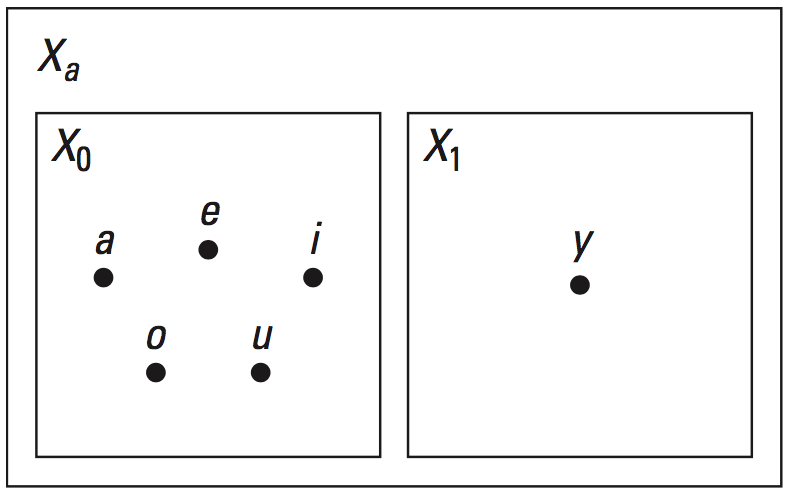
\includegraphics[width=0.5\textwidth]{img/f4-2.png}
	\caption{}
	\label{fig:f4-2}
\end{figure}

Pode-se também aplicar em uma aplicação $ \mathcal{A} $. Se assumirmos que nosso universo é o conjunto de todos os blocos básicos de cada sub-rotina, 

$$ U = \cup_{C \in \mathcal{C}} V(C) $$

então U é as partições de sub-rotinas e chamaremos de partição natural de aplicação onde

$$
\mathcal{S}  = \left \{  
\underbrace{\left \{ b_0, b_1, \dots, b_i \right \}}_{\text{sub-rotine }C_0},
\underbrace{\left \{ b_i, b_{i+1}, \dots, \right \}}_{\text{sub-rotine }C_1},\dots
\underbrace{\left \{ b_j, b_{j+1}, \dots, \right \}}_{\text{sub-rotine }C_{n-1}}
\right \}
$$

Nossa tarefa será reorganizar a partição de blocos básicos e então mapear cada subconjunto de ambos os \textit{hardwares} e \textit{software}. Dessa forma, estamos livres para criar e remover subconjuntos não vazios, e mover blocos básicos ao redor até termos uma nova partição e assim termos um novo resultado $ \mathcal{A}’ = (\mathcal{C}’, \mathcal{L}’) $, inferido a partir da reorganização da partição $ \mathcal{X}’ $. O segundo passo é mapear cada subconjunto de $ \mathcal{X} $ para ambos \textit{hardware} e \textit{software} como é exibido abaixo

$$ 
\mathcal{X}'   = \left \{  
\underbrace{\left \{ b_j, b_{j+1}, \dots, \right \}\left \{ b_k, b_{k+1}, \dots, \right \}\dots}_{\text{software}}
\underbrace{\left \{ b_0, b_1, \dots, b_i \right \} \left \{ b_i, b_{i+1}, \dots, \right \}\dots}_{\text{hardware}}
\right \}
$$



\subsection{Ganho de performance esperado}

Para explicar como performance pode ser utilizado para guiar o particionamento, será utilizado uma métrica simples chamada taxa de execução. É parcialmente motivada pelo fato de que o ganho de performance é relativamente fácil de ser mensurado e por causa de que de todas as métricas comumente utilizadas, \textit{speed up} é frequentemente a mais importante. Diferente do mundo \textit{software} onde tense análise de ordem de complexidade, \textit{hardware} não possui um guia geral para comparação. Ganho de performance para aplicações pode residir em uma acumulação de pequenos ganhos que deveria ser perdido numa aplicação direta na teoria de complexidade. 

Sendo assim, será usado a informação de \textit{profiling} para coletar o tempo total de execução bem com uma fração do tempo gasto em casa sub-rotina. O produto é a aproximação entre o tempo necessário para executar uma porção de aplicação em \textit{software} e usar isso como o tempo que se espera que tomará em futuras execuções. Será utilizado $ s(i) $ para representar o tempo de execução esperado para uma invocação de uma sub-rotina $ i $, ou seja, bloco básico. É uma aproximação para um número de razões, não é o mínimo que depende dos conjuntos de dados de entrada para muitas aplicações. Mesmo assim, existe também exemplos de erros que podem impactar a performance.

Seguindo, precisa-se aproximar o tempo que é uma implementação equivalente em \textit{hardware} que iria tomar. No caso dos blocos básicos, isso é frequentemente mais preciso. Sem fluxo de controle, não presente em blocos básicos, uma ferramenta de síntese pode dar bastante aproximação de acurácia de propagação de tempo. Ou se o recurso é pipelined, o número de estágios é mais precisamente conhecido. Se o recurso inclui fluxo de controle, mas não contém nenhum loop, o caminho mais longo pode ser usado como uma estimativa conservativa. Recursos com um número de variáveis de iterações através de um loop apresentam o maior obstáculo para encontrar um tempo de \textit{hardware} aproximado. Nesse caso, implementação e \textit{profiling} com recurso em \textit{hardware} pode ser a única solução. Independente, assumimos que uma aproximação apropriada $ h(i) $ para o existente tempo de execução em \textit{hardware}.

Finalmente, a interface entre \textit{software} e \textit{hardware} requer tempo e este custo precisa ser contabilizado também. Pode-se aproximar este custo pela aproximação do montante total do estado que necessita ser transferido ou o custo de configuração e latência. Em ambos os caso, são representados por $ m(i) $ para recursos $ i \in \mathcal{H} $.

Taxa de execução é a velocidade na qual um sistema computacional completa uma aplicação, e em um sistema de plataforma FPGA olhamos para o \textit{hardware} para melhorar sua taxa de execução. Esse ganho, no qual comparado com uma solução \textit{hardware} e \textit{software} contra uma solução puramente \textit{software}, é tipicamente mensurada como \textit{speed up}. Utilizamos $ \mathcal{Y} $ para sua representação e isso nos permitira comprar recursos diferentes contra outros para determinar melhores particionamentos. Dessa forma, qualquer subconjunto de blocos básicos que não produzem um ganho de performance, podem ser excluídos geralmente de consideração. Em outras palavras, somente subconjuntos de blocos básicos para qual $ \mathcal{Y} > 1.0 $ são considerados recursos candidatos.

Em geral, não mensuramos taxa de execução, mas ao invés disso, o tempo de execução, que no caso é inverso. Então quando considerando se um conjunto particular de blocos básicos deveriam ser mapeados ao \textit{hardware} ou \textit{software}, estamos interessados em seu ganho em \textit{speed up} ou 

$$ \mathcal{Y} = \frac{\text{hardware speed}}{\text{software speed}} = \frac{\frac{1}{\text{hardware time}}}{\frac{1}{\text{software time}}} = \frac{\text{software time}}{\text{hardware time}} $$

Mais especificamente, estamos interessados no ganho de performance individual de cada recurso e assim, definindo $ \mathcal{Y}(i), i \in \mathcal{C} $

$$ \mathcal{Y}(i) = \frac{s(i)}{h(i) + m(i) } $$

onde $ h(i) $ e $ s(i) $ são o tempo de execução de uma implementação de um recurso $ i $ em \textit{hardware} e \textit{software}. A função $ m(i) $ é o tempo que se leva para sincronização, estado preso, ou seja, o tempo que leva para guiar um dado entre o processador e o item reconfigurável.

Assumindo por um momento que usaremos esse recurso separado em nosso design, deve-se questionar sobre o quão rápido é a aplicação. Isso é dependente em ambos o ganho de performance do recurso e o qual frequentemente é utilizado no design referencial de \textit{software}. Pode-se ter uma fração do tempo gerado em um recurso particular $ f(i) $ a partir de informações de \textit{profile}. Então, o \textit{speed up} da aplicação no geral será

$$ \Gamma = \left [ (1 - f(i)) + \frac{f(i)}{\mathcal{Y}(i)} \right ]^{-1}  $$

A inversão representa que estamos movendo entre tempo de execução e taxa de execução para manter o sentido de ganho de performance.

A partir dessa equação, podemos observar que aumentando a velocidade do \textit{hardware} de um único recurso tem-se menos e menos impacto na performance da aplicação a medida que sua frequência decresce. Para aumentar a performance sistêmica de uma aplicação no geral, também queremos olhar sobre uma outra dimensão: aumentando o sistema com múltiplos recursos que aumentará a performance de componentes individualmente assim como aumentando a fração agregada de tempo gasto em \textit{hardware}. Reconhecendo isso, queremos computar o \textit{speed up} de múltiplos recursos em \textit{hardware}, ou seja, quer-se avalizar o ganho sistêmico de um conjunto de recursos $ \mathbb{D} $ onde cada membro do conjunto contribui à performance do sistema baseado na fração do tempo gasto em cada característica. Para estimar a performance desta partição, podemos adicionar recursos e rearranjar os termos para ter um ganho de performance esperado no geral

$$ \Gamma (\mathbb{D} = \left [ 1 + \sum _{i \in \mathbb{D}} (\frac{f(i)}{\mathcal{Y}(i)} – f(i)) \right ]^{-1} $$



\subsection{Considerações de Recursos}

Seguindo a equação exibida, se tentaria adicionar recursos na abordagem $\sum_i f_i$. Em outras palavras, seria implementar tudo em \textit{hardware} para maximizar a performance, ignorando todos os custos de desenvolvimento e recursos limitados. Num FPGA, há um número finito de recursos disponíveis para implementação de circuitos em \textit{hardware}. Tais recursos são limitados e a maioria das aplicações realísticas irão exceder esse limite disponível. Um meio de aproximação de recursos é contar o número de células lógicas requeridas para cada recurso. Um chip que terá um valor escalar $ r_{FPGA} $ que representa o total de números de células lógicas disponíveis. Então $ r(i) $ pode ser usado para representar a quantidade de células lógicas requeridas por cada recurso $ i $. Uma simples relação 

$$ \sum_{i \in \mathbb{D}} r(i) < r_{FPGA} $$

restringe quão largo $ \mathbb{D} $ pode crescer.

Sabendo que dispositivos modernos são heterogêneos, uma típica plataforma FPGA tem múltiplos tipos de recursos além de células lógicas como memória, blocos DSP, etc. Sendo assim, um vetor seria uma melhor representação

$$ 
\vec{r}_{FPGA} =
\begin{pmatrix}
r_0\\ 
r_1\\ 
\dots \\
r_{n-1}
\end{pmatrix}
$$

Também promovemos a função de requerimentos de recursos para um vetor onde $ \vec{r}(i) $ representa o recurso requerido pelo recurso $ i $. Assim, a nova equação de restrição de recurso é similar 

$$ \sum_{i \in \mathbb{D}} \vec{r}(i) < \vec{r}_{FPGA} $$

onde $ \mathbb{D} $ é o conjunto de recurso incluídos no design.

Infelizmente, esse modelo não toma conta o fato de que alguns recursos alocados podem interferir em outros além de que a estimativa de performance é frequentemente baseada na suposição que recursos são próximos um do outro e recursos de rotas não são parte integral do modelo.



\subsection{Abordagem Analítica}

Já descrito as ferramentas matemáticas necessárias para descrever o problema fundamental do particionamento, pode-se então, primeiramente descrever formalmente o problema em termos de variáveis e descrever um algoritmo para encontrar uma solução aproximada.



\subsubsection{Declaração do problema}

A ideia básica é encontrar um particionamento para todos os blocos básicos de uma aplicação e então separá-los em \textit{hardware} e \textit{software}. Formalmente, procura-se por uma partição $ \mathcal{P} $ de todos os blocos básicos $ U $ de uma aplicação

$$ U = \cup_{C \in \mathcal{C}} V(C) $$

Um subconjunto, $ \mathbb{C} \subseteq U $ onde $ C $ é um vértice de um grafo $ A = (C, L) $ de um design referencial de \textit{software}, é chamado conjunto de candidatos e contem todos os recursos arquiteturais potenciais, ou seja, o subconjunto de $ U $ que é esperado para melhorar a performance do sistema se implementado em um \textit{hardware} reconfigurável. Devido ao limite de recursos, deve-se refinar para o subconjunto $ \mathbb{D} \subseteq \mathbb{C} $ que maximiza nosso métrica de performance

$$ \Gamma ( \mathbb{D}) \text{é maximizado, e } \\ 
\sum_{i \in \mathbb{d}} \vec{r}(i) < \vec{r}_{FPGA}
$$

Algoritcamente, uma abordagem desse problema seria encontrar todas as partições de $ U $, sintetizando e \textit{profiling} cada partição, e então, quantitativamente avalizar cada $ \Gamma $, mas uma aplicação simples que utilizaria cerca de 10 mil blocos básicos, seria mais que $ 10^7 $, significando que o número de partições seria aproximadamente $ 2^{10^{7}} $ e por isso será discutido métodos heurísticos para tal.



\subsubsection{Heurística}

O problema de particionamento é essencialmente uma questão indireta de manipulação de parâmetros $ f(i) $ e $ \gamma(i) $ pelo rearranjo do particionamento $ \mathcal{X} $. Então seleciona-se os elementos de $ X $ que satisfaz as restrições de recurso e maximiza a performance do sistema $ \Gamma $. A heurística pode ser aplicada informalmente para iniciar a partição natural por design referencial de \textit{software}, ou seja, utiliza-se as sub-rotinas de uma aplicação original. Utilizando a ferramenta de \textit{profiling} é listado as sub-rotinas em ordem decrescente em tempo e verificado as que possuem maior valor $ f $. O valor de $ \gamma $ será estimado pela performance esperada a partir da implementação em \textit{hardware} e ao final, tem-se um ganho estimado do sistema para cada sub-rotina.



Em seguida, quer-se manipular iterativamente a partição $ \mathcal{X} = \{ X_0, X_1, ...\} $ criando um novo subconjunto de blocos básicos por meio de operações de casamento e movimentações de blocos. A ideia é procurar mudanças que podem aumentar a fração $ f $ ou o valor de $ \gamma $.



\subsubsection{Fração do Tempo de Execução}

Uma forma de aumentar fração de tempo gasto em uma sub-rotina é tornando maior seu recurso. Isso pode ser alcançado procurando por relações no grafo de chamadas ou, após a manipulação, procurando por relacionamentos no grafo de fluxo de controle que conecta subconjuntos. Por exemplo, supondo que uma aplicação gaste $ 0.5 \% $ do seu tempo, $ f(i) = 0.005 $ numa sub-rotina A e $ 0.025\% $ em uma sub-rotina B e C. A fração de tempo gasto em A pode ser duplicado pelo casamento de A, B e C, entretanto, isso possui seu preço. Geralmente, aumenta-se o número de recursos utilizados e também pode aumentar no tamanho do subconjunto do sistema, decrescendo sua performance.



\subsubsection{Ganho de Performance}

Para aumentar o ganho de recurso $ \gamma (i) $ necessita-se verificar o grafo de fluxo de controle do recurso e avaliar se uma mudança o tornará mais sequencial ou paralelo. Frequentemente, algoritmos que são inerentemente sequenciais possuem melhor performance em processador por este não ter a sobrecarga de configurações de transistores e de possuírem melhor gerenciamento de energia nessas circunstâncias. Simplesmente adicionar blocos básicos pode criar um efeito indesejável de aumentar o comportamento sequencial, reduzindo o $ \gamma $ e criando um recurso menor, pode aumentar seu ganho. Assim, tendo uma sub-rotina $ X $ e quebrando-a em duas sob-rotinas $ X – X' $ e $ X' $, onde a sub-rotina $ X – X' $ invoca $ X' $, então se $ X' $ pode ser melhorado em nível de \textit{hardware} deixando a parte sequencial em $ X – X' $ então $ \gamma $ de $ X' $ será maior e necessitará de mais recursos. Assim, supondo uma sub-rotina tome $ 93\% $ de tempo e provê ganho de $ \gamma = 2 $ então a aplicação terá performance de $ \Gamma = 1.869 $. Entretanto, se uma parte da sub-rotina pode ser extraída aumentando o paralelismo, então é possível que a performance possa chegar a um valor de $ 10 $, $ \gamma = 20 $ enquanto o tempo decresce para $ 83\% $. Esse particionamento gera um \textit{\textit{speed up}} de $ \Gamma = 4.739 $.


Com isso é importante notar que qualquer mudança no subconjunto pode afetar a performance para melhor ou pior. Em geral, heurísticas trabalham examinando os grafos da aplicação e então fazendo mudanças incrementais ao subconjunto de uma partição. Tais mudanças são guiadas pela tentativa de aumentar o tempo gasto em uma sub-rotina não aumentando dramaticamente seus recursos ou decrescendo sua performance; e tentando aumentar a performance sem reduzir o tempo gasto em uma sub-rotina.



\section{Comunicação}

Ao realizar o particionamento, deve-se criar uma comunicação entre os componentes e com isso deve-se discutir o número de questões relacionadas ao estado de comunicação sobre os limites do particionamento e o mecanismo para controle de transferência entre ambos os níveis. Um exemplo disso é uma sub-rotina que realiza a correção de erro bit a bit. É esperado que, como existem operações em bits, a sub-rotina possua melhor desempenho ao ser implementada em \textit{hardware}, tornando-a uma candidata. Inicialmente é posta como uma candidata pois os recursos possuem números limitados e talvez ela não faça parte da decomposição mais benéfica. Uma vez implementada em \textit{hardware}, deve-se realizar a interação entre o recurso e o processador. Sabendo que existem abundância em interfaces padronizadas, em FPGA é possível utilizar uma interface pré-definida ou criar uma nova para cada recurso e essa questão é crucial pois a comunicação também define a performance do sistema.



Adicionar um recurso requer que o processador e o recurso mantenham constante visão dos dados da aplicação. O interfaceamento é o que permite o recurso e o processador comunicar mudanças de estado e é necessário para continuar um dado de aplicação consistente. No desenvolvimento de design referencial de \textit{software}, o programador não especifica essas questões. A especificação utiliza um modelo sequencial no qual pode não expressar qualquer concorrência ou hierarquia de memória. Quando a consistência não é explicitada na interface de comunicação, o sistema possui grande risco de produzir resultados incorretos e para isso será discutido a invocação e coordenação de recursos.



\subsection{Invocação e Coordenação}

Da mesma forma que modelos de computação sequencial e \textit{multithread} podem realizar invocações de sub-rotinas, o mesmo pode ser realizado em \textit{hardware} com o codinome de política de coordenação. Em nível de \textit{hardware} existe diferenciações pois neste não existe controle de de \textit{thread} mas geralmente possui somente um controlador que habilita ou não o recurso para processamento. Muitas máquinas de estado têm uma ordem de estados \textit{idle} e a transferência de controle pode ser a sua ativação. Existe três abordagens para coordenar um \textit{hardware} e \textit{\textit{software}} e serão descritas a seguir.



\subsubsection{Modelo de Coprocessador}

Também conhecido como modelo \textit{go/done} ou modelo cliente/servidor, o modelo coprocessado é similar a sub-rotina chamada acoplamento. Neste modelo, o \textit{hardware} fica em estado neutro, esperando fornecer um serviço para o processador. O processador envia um sinal de início e espera o resultado. Neste modelo, todo recurso em \textit{hardware} deve ter o estado \textit{idle} já definido em design e padronizado para iniciar em modo desligado. Um item importante nesse sistema é saber manusear o tempo enquanto o recurso está operando algumas formas em especiais serão citadas a seguir.



\paragraph{Fixando o Tempo}

Para recursos de pequeno porte que possuem um tempo fixo, o mecanismo mais eficiente é o processador realizar um número de instruções ``\textit{no-op}'' para que em seguida possa receber o resultado sempre checando o sinal \textit{done}.



\paragraph{\textit{Spin-Lock}}

Quando o total de tempo é desconhecido, utiliza-se mecanismo de \textit{spin-lock}. É um processo conhecido como \textit{pooling} onde o processador fica num processo repetitivo de questionamento ao recurso se sua operação já foi finalizada.



\begin{verbatim}
// Simple y = m*x + b Example 
invoke_hw(m, x, b); 
while(!done) {
    done = check_done_signal(); 
}
y = retrieve_results();
\end{verbatim}



\paragraph{Bloqueio}

A forma tradicional utilizada nesta situação é tratar o recurso como um dispositivo de I/O. O sinal \textit{done} pode ser tratado como uma interrupção ao processador no qual permite o recolhimento do resultado.

\begin{verbatim}
// Simple y = m*x + b Example 
invoke_hw(m, x, b);
yield();
y = retrieve_results();
\end{verbatim}



\paragraph{Solução Especial para o Modelo de Coprocessador}

A transferência de um estado de \textit{hardware} para \textit{software} é muito das vezes impraticável. Determinando primeiramente os métodos, o algoritmo foca nos locais mais prováveis para a extração de recursos. 

Um grafo de chamadas estático é construído e a recursão é utilizada para detectar componentes fortemente conectados do grafo e retirados de consideração.


\begin{figure}[h] \centering
	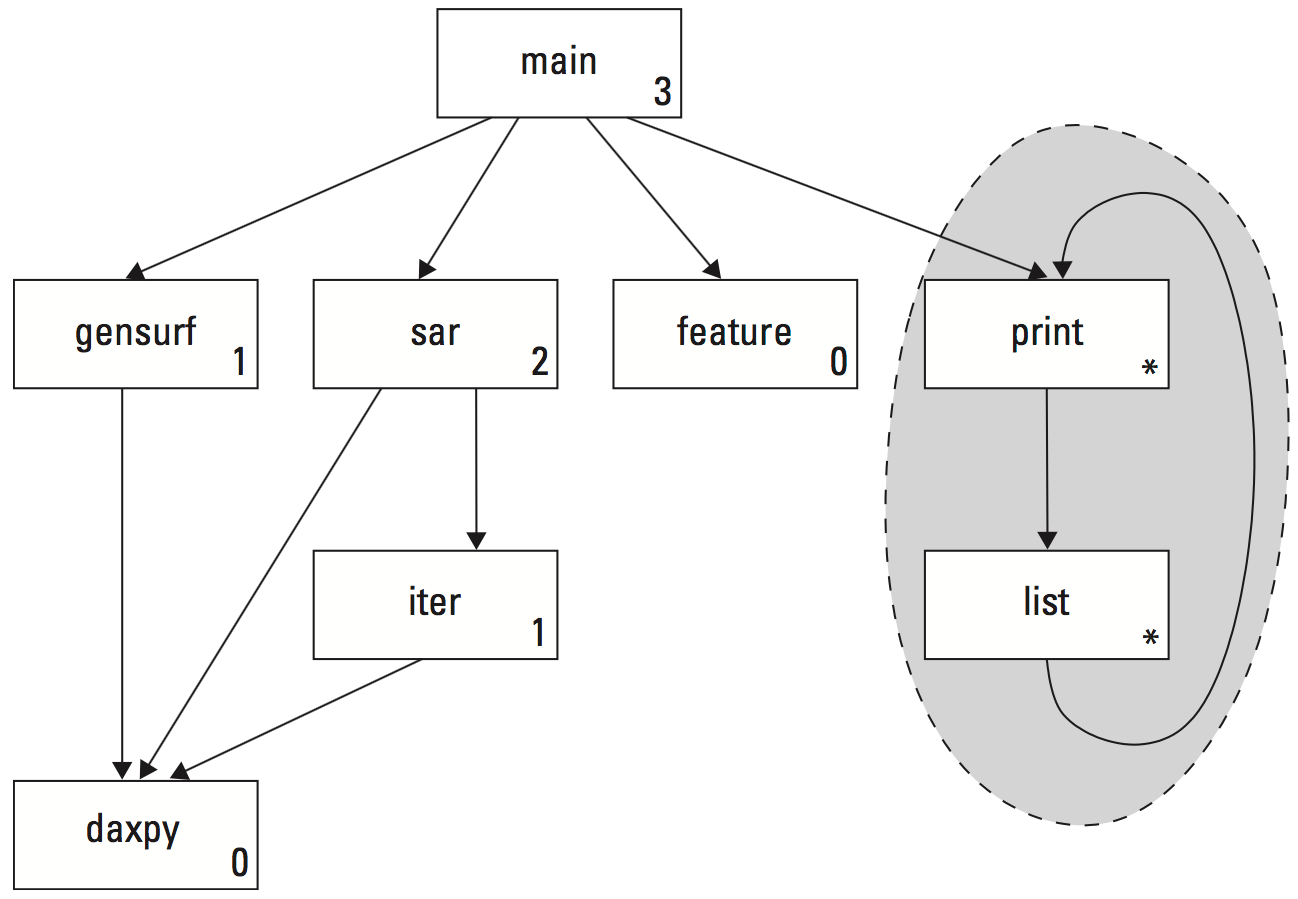
\includegraphics[width=0.8\textwidth]{img/f4-4.png}
	\caption{}
	\label{fig:f4-4}
\end{figure}

O exemplo da Figura \ref{fig:f4-4} mostra que as funções \texttt{print} e \texttt{list} formam um componente fortemente conectado e são marcados com um *. Em seguida, os vértices restantes de $ G $ são assinalados por uma regra ordinal,

$$
\text{ord}(u) = 
\left\{\begin{matrix}
0 & \text{se nó} u \text{é uma folha} \\ 
\underset{(u,v) \in E(G)}{\max} \{ \text{ord}(v) \} + 1 & \text{caso contrário}
\end{matrix}\right.
$$



\subsubsection{Modelo \textit{Multithread}}

Além do modelo coprocessado, tem-se o modelo \textit{multithreads} que emerge como uma importante técnica de programação utilizada até em computadores com multiprocessadores. Neste modelo, o paralelismo natural do \textit{hardware} é conhecido e o designer reconhece que o processador e os componentes executam continuamente. A coordenação desses componentes é manuseada por comunicações primitivas que tem sido desenvolvidas por processo concorrentes como semáforos, mensagens e outros. Cada \textit{hardware} é considerado um componente que executa como uma \textit{thread} paralela e o sistema de semáforos é utilizado para deixar o sistema consistente e assim, ao invés de bloqueado, o \textit{hardware} conceitualmente fica em bloqueio esperado pelo semáforo ou por uma mensagem.



\subsubsection{Modelo de Rede em Chip}

Este modelo investiga o estado distribuído completamente e depende da troca de mensagem para explicitar o estado. A coordenação é implícita com a transferência de estado. Como é assumido que o design referencial de \textit{software} foi construído com comandos de troca de mensagem explícita, não se considera em um manual de sistemas embarcados. Entretanto, tem-se visto que técnicas de alta-performance continuam filtrando-se para o nível de sistemas embutidos.



\subsection{Transferência de Estado}

Manter estado consistente sobre dispositivos FPGA e processadores é um desafio. Isso pois, cada FPGA tem sua própria hierarquia de memória independente, estados são amplamente distribuídos no design, e há ampla variedade de interconexões entre FPGA e processadores significando menos estados para serem transferidos e grande variedade de mecanismos disponíveis. Para entender melhor deve-se definir dois conceitos sendo eles estado afetado e preso ajudando a decidir quais partes do estado da aplicação necessitam de ser explicitamente comunicados entre processador e recurso.



\subsubsection{Estado Afetado}

Na computação alguns estados são independentes pela construção e não precisam de ser transferidos. Retirando tais estados, restam somente os estados afetados no qual são os dados da aplicação que, durante a transferência de controle, podem ser modificados ou litros por um recurso ou processador, necessitando de ser consistente.



Estados afetados podem existir em grande escala principalmente quando arranjos, estruturas de dados complexas ou ponteiro estão envolvida e podem ser acessados de várias formas possíveis e geralmente não é possível saber se dois ponteiros estão apontando para um mesmo endereço.



\subsubsection{Estado Preso}

Quando parte da hierarquia de memória é compartilhada, nem todo o dado tem que ser explicitamente transferido. Computadores modernos são construídos com quantidade significativa de memória pode ser utilizada como parte de estado sem a atualização da memória primária. Compiladores naturalmente utilizam toda a vantagem de registradores para armazenar estados, implementações em \textit{hardware} incorporam dados ao longo do projeto e seus registradores e \textit{flip-flops} possuem valores intermediários entre ciclos de \textit{clock} dentro do projeto. O estado de uma aplicação é armazenado em várias partes do sistema. Para um recurso implementar parte de uma aplicação, precisa-se integrar com parte do estado. Esse pode ser considerado mais facilitado pelo fato de que o estado está localizado em um espaço comum mas se um estado está localizado num registrador ou em uma cache de um processador, ele não pode ser acessado pelo sistema externo e, neste caso, o estado encontra-se preso e deve ser explicitamente transmitido pela interface.



\subsubsection{Problema de Transferência de Estado}

Estados afetados que são presos necessitam de ser explicitamente comunicados e é feito por um processo chamado \textit{marshaling}, realizando o processo de \textit{marshaling} grupos de elementos de um estado afetado de uma aplicação em registros lógicos que são explicitamente transferidos. Tendo a premissa que o processador tem o controle inicial, tem-se quatro tipos de registros que podem ser utilizados. Os dois primeiros são utilizados para iniciar e outro para finalizar a transferência de um conjunto de elementos para o recurso sendo eles \textit{Type-I} e \textit{Type-F}. Os outros dois tipos de \textit{marshal} são utilizados repetidamente e são utilizados quando o recurso é invocado, \textit{Type-CI}, e quando é completado \textit{Type-CO}. Um exemplo da diferença entre \textit{Type-F} é quando se tem um \textit{core} que acumula um valor em uma variável global. O registro \textit{Type-F} seria utilizado para ler o valor da variável após sua última invocação \textit{Type-CO}.



Um processo de tradução pode ser incorporado com o \textit{marshaling}, sendo o exemplo o processo de conversão de ponto flutuante para fixo. O grupo de elementos é lógico pelo fato do \textit{assembly} não significar estritamente que os elementos são copiados para uma memória de locação contínua. 



A forma mais simples de transferir estados são copiando os registros, parar o processador enquanto o recuso processa. Este é chamado de empurrar (\textit{push}) os dados no qual transmite o dado antes da transferência do controle. Caso registro já existe e é conhecido, é feito a transferência de controle e o recurso realiza o puxar (\textit{pulls}) dos dados. Situações onde o estado afetado é maior que o dado a ser utilizado, utiliza-se de interfaces.



Em geral, a escolha da transferência por instância ou por continuação é determinada por uma meta do recurso. Instâncias são utilizadas quando deseja-se reduzir a latência de tarefas e transferir pequenos registros. Continuações são para aumentar a vazão de dados e a redução de latência não é possível ou não suficiente boa. Esta geralmente envolve a configuração de transferências DMA e a incorporação de \textit{buffers} FIFO no qual pode aumentar a área e em algumas situações a latência.



As melhores implementações em \textit{hardware} utilizam formatos diferentes de estruturas de dados. Traduções são item integral para dados \textit{marshal}.



Esclarecido os conceitos fundamentais, será descrito a abordagem formal para o problema de particionamento.



\section{Questões Práticas}

\subsection{Questões de \textit{Profiling}}

Uma suposição não adequada com a formulação analítica é que ela usa informação de \textit{profile} para aproximar o tempo de fração que uma aplicação gasta em uma sub-rotina ou bloco básico, mas no entanto, várias situações podem gerar resultados enganosos.



\subsubsection{Execução Dependente de Dados}

Quanto um simples conjunto de dados não representa o tempo gasto de cada sub-rotina quando este é alterado a sub-rotina não terá mudanças substanciais com a mudança do dado de entrada. A detecção da situação onde um único conjunto de dados não é representativo torna a situação difícil e requer que o designer do sistema compreenda a operação fundamental da aplicação como é o caso da análise de complexidade das rotinas. É possível analisar esses casos com alguns métodos sendo a análise manual dos algoritmos e suas operações básicas, a coleta de informações \textit{profiling} baseado em diferentes conjuntos de dados ou mesmo a tentativa de separar a aplicação talvez ao longo dos limites do módulo e fazer o \textit{profile} de cada módulo independente.



\subsubsection{Comportamento Correlacionado}

Outra questão surge em aplicações que explicita o uso de eventos cronometrados. Muitos \textit{profile} assumem que a aplicação fará um progresso estável em direção à solução mas algumas aplicações incorporam o tempo. Sistemas de \textit{profiles} usam um temporizador de intervalo para amostrar o contador de programas dependendo da aplicação para não serem correlacionados estatisticamente com o temporizador. No entanto, se a aplicação possui operações executando em tempos regulares, periódicos, então os resultados do \textit{profiling} podem ser considerado enganosos. Por exemplo, se uma aplicação é executada a cada 10ms e a amostragem é feita a cada 10ms, então o \textit{profiler} não fornecerá dados concretos referentes ao sistema.



\subsubsection{Comportamento Faseado}

Sobre a totalidade de sua execução, o controle se move entre \textit{clusters} de operações relacionadas, isso é, a execução de uma aplicação exibida localmente. Como um exemplo, consideremos uma aplicação que possui três rotinas. Assumindo que cada possui $ 33\% $ de tempo de execução, e que cada tem a possibilidade de ter um \textit{speed up} de 50\% e postas de forma ordenada da primeira à última. Se existe espaço somente para uma rotina em recursos de FPGA, então o \textit{speed up} máximo será de 12\%. Mas se o comportamento faseado é suportado pelo design de sistema, então há mais opções. Um é olhar procurar itens em comum sobre os três \textit{cores} e uma segunda é um \textit{hardware} multiplexado por tempo. Não há abordagens automáticas para esse.



\subsubsection{Efeitos de I/O}

\textit{Profiles} não contam tempo de I/O tais como acesso ao espaço de usuário e dispositivos realizando algum procedimento de busca ou ação.



\subsubsection{Números de Chamada}

\textit{Profiles} entretanto continuará a calcular quando sub-rotinas são invocadas. É importante ter noção o quanto uma sub-rotina é invocada.



\subsection{Estrutura de Dados}

Design de referência de \textit{software} naturalmente reflete um viés em relação às implementações em \textit{software}. Isso é compreensível, já que a programação é ensinada no contexto de modelo de computação sequencial ordinário. Com esses modelos, a diferença entre 

\begin{verbatim}
while( i!=NULL ) {
  proc(i) ;
  i = i->next ;
} 
\end{verbatim}
e 
\begin{verbatim}
while( i<n ) {
 proc(x[i]) ;
 i=i+1;
}
\end{verbatim}

é insignificante já que ambos tomam $ \mathcal{O}(n) $ passos, mas em nível de \textit{hardware} o último pode ser mais desejável sendo no mínimo, uma ampla janela de pré-busca é possível. Se pudermos determinar que, em várias iterações do ciclo, cada \texttt{proc(x[i])} é independente, então pode-se melhorar o design por meio de \textit{pipeline} ou paralelismo regular.

O design de referência de \textit{software} serve como extremamente bem como uma especificação, mas se executar um \textit{profile} do design de referência, não será capturado os benefícios da implementação pois esses benefícios provêm de alterações algorítmicas e são improváveis de serem reveladas por técnicas automáticas. Consequentemente, cai sobre o designer de sistema compreender ambos o algoritmo de \textit{software} implementado no design referencial e como pode ser re-implementado em \textit{hardware}.

Há vários formas comuns de estruturas de \textit{software} que pode ser rearranjadas para produzir melhor design de \textit{hardware}. Estruturas de dados que utilizam ponteiro como listas encadeadas, árvores, etc. podem ser representadas por uma estrutura ``\textit{flat}'' como vetores e arranjos produzindo acesso regular em memória que podem ser pré-buscadas subsequentemente ou utilizadas em \textit{pipeline}. Outra forma de ganho de performance é no tamanho de bit. Programadores de \textit{software} geralmente assumem um valor fixo, mesmo que utilizem somente poucos bits de informação. Enquanto \textit{software} tem caminho de dados fixos e relativamente baixa largura de banda entre componentes, \textit{hardware} se destaca no gerenciamento de largura de bits arbitrárias sendo possível alavancar grande largura de banda fornecida pela interconexão programável do FPGA.



\subsection{Manipulando Tamanho de Recurso}

A mudança mais simples envolver quebrar uma sub-rotina em sub-rotinas menores fazendo com que o recurso em \textit{hardware} fique menor e mais fácil de ser implementado.



Há três momentos que agregar sub-rotinas são necessárias. Se duas sub-rotinas tomam 25\% cada uma do tempo da aplicação, então elas são candidatos fortes para a implementação em \textit{hardware}. No entanto, se for implementado individualmente, cada uma invoca o custo da sua interfaceação. Se há três sub-rotinas relacionadas (uma invocando a próxima), então a combinação delas pode reduzir o custo de invocações. Entretanto, o custo da interface não é sempre insignificante e vale a pena o esforço do usuário para investigar a situação.



Qualquer outra mudança é substancial. Frequentemente, implementação em \textit{hardware} tem performance significativa por ter formato de dados de dados específicos da aplicação. Para que o \textit{software} seja mais eficiente nos formato de dados não padronizados, programadores irão investir em estruturas de dados que não são bem mapeadas para o \textit{hardware}. Assim, vale a pena olhar para o propósito e considerar a substituição de estruturas de dados para melhor explorar o \textit{hardware}.


	%\input{tex/chap2}
	%\input{tex/chap3_final}
	%\input{tex/chap4}
	%\input{tex/chap5}
	%\input{tex/chap6_final}
\end{mainmatter}

%% Produce the appendices
\begin{appendices}
\begin{flushleft}

\end{flushleft}
	  \selectlanguage{brazilian}
  	%\input{tex/appendices}
\end{appendices}
\let\cleardoublepage\clearpage
%% Produce the un-numbered back matter (e.g. colophon,
%% bibliography, tables of figures etc., index...)
\begin{backmatter}
	%\input{tex/backmatter}
\end{backmatter}

%% Close
\end{document}
